\documentclass[conference]{IEEEtran}
\IEEEoverridecommandlockouts
% The preceding line is only needed to identify funding in the first footnote. If that is unneeded, please comment it out.
\usepackage{cite}
\usepackage{amsmath,amssymb,amsfonts}
\usepackage{graphicx}
\usepackage{textcomp}
\usepackage{xcolor}
\usepackage{booktabs}
\usepackage{multirow}
\usepackage{array}
\newcolumntype{L}[1]{>{\raggedright\arraybackslash}p{#1}}
\usepackage{tikz}
\usetikzlibrary{positioning,arrows.meta,fit}
\usepackage{pdflscape}
\usepackage[hidelinks]{hyperref}
% ---------------------------------------------------------------------------
% Click-to-enlarge figures. Every figure links to a full-page copy at the end
% of the PDF; each full-page copy links back. Set \fullfigsfalse to remove
% the full-size pages and the links (for example, for a page-limited submission).
% ---------------------------------------------------------------------------
% Pop-up mode (\popupfigstrue): clicking a figure opens an enlarged copy on top
% of the same page; clicking the copy closes it. Pop-ups need a PDF viewer with
% layer support (Adobe Acrobat Reader); in pop-up mode the full-size pages are off.
\newif\iffullfigs
\fullfigstrue
\newif\ifpopupfigs
\popupfigsfalse
\ifpopupfigs\fullfigsfalse\fi
\ifpopupfigs
  \usepackage{ocgx2}
\fi
\newlength{\popw}\setlength{\popw}{\dimexpr\paperwidth-2cm\relax}
\ifpopupfigs
  \usepackage{zref-abspage,zref-user}
\fi
\makeatletter
\newcommand{\pop@list}{}
% Draws, on top of everything else on the page, the pop-ups of the figures placed there.
\newcommand{\pop@draw}[1]{%
  \ifnum\zref@extractdefault{popat:#1}{abspage}{0}=\value{abspage}\relax
    \put(\strip@pt\dimexpr0.5\paperwidth\relax,-\strip@pt\dimexpr0.5\paperheight\relax){\makebox(0,0){%
      \begin{ocg}[printocg=never]{Enlarged #1}{pop:#1}{0}%
      \toggleocgs{pop:#1}{\fcolorbox{gray!60}{white}{\parbox{\popw}{\centering
        \csname pop@big@#1\endcsname\par\smallskip
        {\small\textcolor{blue!60!black}{Click the figure to close}}}}}%
      \end{ocg}}}%
  \fi}
\ifpopupfigs
  \AddToHook{shipout/foreground}{\pop@list}
\fi
\newcommand{\clickfig}[3]{% #1 label, #2 figure as printed, #3 enlarged copy
  \ifpopupfigs
    \toggleocgs{pop:#1}{#2}\zlabel{popat:#1}%
    \expandafter\gdef\csname pop@big@#1\endcsname{#3}%
    \g@addto@macro\pop@list{\pop@draw{#1}}%
  \else\iffullfigs
    \hypertarget{back:#1}{}\hyperlink{full:#1}{#2}%
  \else #2\fi\fi}
\makeatother
\newcommand{\enlarge}{\iffullfigs\ \textit{(Click to enlarge.)}\fi\ifpopupfigs\ \textit{(Click to enlarge.)}\fi}
\newcommand{\fullfig}[3]{% #1 label, #2 content, #3 title
  \begin{center}
  \hypertarget{full:#1}{}%
  {\large\textbf{Fig.~\ref{#1}.} #3}\par\medskip
  #2\par\medskip
  \hyperlink{back:#1}{\textcolor{blue!60!black}{$\leftarrow$ Back to Fig.~\ref{#1} in the text}}
  \end{center}
  \clearpage}
\newcommand{\fullfigL}[3]{% wide figures: a landscape page
  \begin{landscape}
  \begin{center}
  \hypertarget{full:#1}{}%
  {\large\textbf{Fig.~\ref{#1}.} #3}\par\medskip
  #2\par\medskip
  \hyperlink{back:#1}{\textcolor{blue!60!black}{$\leftarrow$ Back to Fig.~\ref{#1} in the text}}
  \end{center}
  \end{landscape}}
\def\BibTeX{{\rm B\kern-.05em{\sc i\kern-.025em b}\kern-.08em
    T\kern-.1667em\lower.7ex\hbox{E}\kern-.125emX}}

\newcommand{\frameworkdiagram}{%
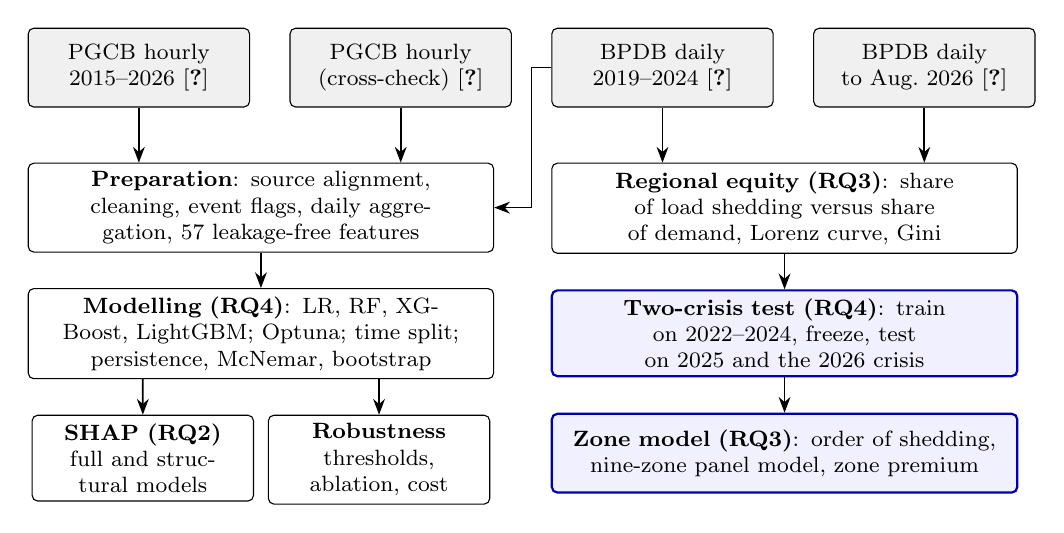
\begin{tikzpicture}[
  font=\footnotesize,
  box/.style={draw, rounded corners=2pt, align=center, minimum height=1.0cm, text width=2.6cm, inner sep=3pt},
  data/.style={box, fill=gray!12},
  nov/.style={box, draw=blue!70!black, fill=blue!6, line width=0.8pt},
  arr/.style={-{Stealth[length=2mm]}, semithick},
  node distance=0.45cm and 0.5cm]
\node[data] (d1) {PGCB hourly\\2015--2026~\cite{shekh2026}};
\node[data, right=of d1] (d2) {PGCB hourly\\(cross-check)~\cite{ucipgcb}};
\node[data, right=of d2] (d3) {BPDB daily\\2019--2024~\cite{hossain2025}};
\node[data, right=of d3] (d4) {BPDB daily\\to Aug.\ 2026~\cite{islam2026}};
\node[box, below=0.7cm of d1, xshift=1.55cm, text width=5.7cm] (prep) {\textbf{Preparation}: source alignment, cleaning, event flags, daily aggregation, 57 leakage-free features};
\node[box, below=of prep, text width=5.7cm] (model) {\textbf{Modelling (RQ4)}: LR, RF, XGBoost, LightGBM; Optuna; time split; persistence, McNemar, bootstrap};
\node[box, below=of model, xshift=-1.5cm, text width=2.6cm] (shap) {\textbf{SHAP (RQ2)}\\full and structural models};
\node[box, below=of model, xshift=1.5cm, text width=2.6cm] (rob) {\textbf{Robustness}\\thresholds, ablation, cost};
\node[box, below=0.7cm of d3, xshift=1.55cm, text width=5.7cm] (eq) {\textbf{Regional equity (RQ3)}: share of load shedding versus share of demand, Lorenz curve, Gini};
\node[nov, below=of eq, text width=5.7cm] (two) {\textbf{Two-crisis test (RQ4)}: train on 2022--2024, freeze, test on 2025 and the 2026 crisis};
\node[nov, below=of two, text width=5.7cm] (zone) {\textbf{Zone model (RQ3)}: order of shedding, nine-zone panel model, zone premium};
\draw[arr] (d1) -- (d1 |- prep.north);
\draw[arr] (d2) -- (d2 |- prep.north);
\draw[arr] (d3) -- (d3 |- eq.north);
\draw[arr] (d4) -- (d4 |- eq.north);
\draw[arr] (prep) -- (model);
\draw[arr] (model.south) ++(-1.5,0) -- (shap.north);
\draw[arr] (model.south) ++(1.5,0) -- (rob.north);
\draw[arr] (eq) -- (two);
\draw[arr] (two) -- (zone);
\draw[arr] (d3.west) -- ++(-0.25,0) |- (prep.east);
\end{tikzpicture}}

\begin{document}

\title{Two Crises, Nine Zones: Explainable Early Warning of Load Shedding in Bangladesh}

% ---------------------------------------------------------------------------
% AUTHORS: replace the placeholders. List authors left to right; the mentor
% or supervisor is usually the last author. Add or remove \and blocks as needed.
% ---------------------------------------------------------------------------
\author{
\IEEEauthorblockN{Md. Shoyaif Rahman}
\IEEEauthorblockA{
\textit{Department of Computer Science and Engineering} \\
\textit{University of Information Technology and Sciences (UITS)} \\
Bangladesh \\
0432310005101050@uits.edu.bd
}
\and
\IEEEauthorblockN{Shad Ahmed\\(Supervisor)}
\IEEEauthorblockA{
\textit{Department of Computer Science and Engineering} \\
\textit{University of Information Technology and Sciences (UITS)} \\
Bangladesh \\
shad.ahmed@uits.ac.bd
}}

\maketitle

\begin{abstract}
Bangladesh has faced recurring load shedding since mid-2022, driven largely by fuel-supply shortfalls, yet earlier machine-learning studies of this shedding have not compared their models with a persistence baseline, tested them across separate crises, or examined how shedding is distributed across regions. This study examines whether interpretable machine learning can warn of next-day national load shedding above 100 MW and who bears it. We combined hourly Power Grid Company of Bangladesh records (2015--2026) with daily Bangladesh Power Development Board reports (2019--2026), built 57 leakage-free features, and tuned logistic regression, random forest, XGBoost and LightGBM with time-ordered cross-validation. Models were compared with a persistence baseline, explained with SHAP, and tested out of sample on a calm year (2025) and a new crisis (January to August 2026). On the 2025--2026 test period, XGBoost ranked risk better than persistence (PR-AUC 0.832 versus 0.608) and correctly called 37.6\% of transition days, but its accuracy gain (0.810 versus 0.785) was not statistically significant (McNemar p-value 0.19). A model frozen after the 2022--2024 crisis reached 0.893 accuracy in the 2026 crisis against 0.860 for persistence (p-value 0.12), whereas monthly retraining did worse. SHAP indicated higher risk when next-day maximum temperature exceeded about 32.5 degrees Celsius, demand exceeded about 12,800 MW, and a demand--supply gap was present. Shedding was unequal: Mymensingh held 8.4\% of demand but 27.5\% of load shedding, and absorbed 65\% of national shedding on low-shortfall days. Interpretable gradient boosting can support early warning and equity monitoring, although its gains over simple rules are modest.
\end{abstract}

\begin{IEEEkeywords}
load shedding, Bangladesh power system, gradient boosting, SHAP explainability, early warning, energy equity
\end{IEEEkeywords}

% ===========================================================================
\section{Introduction}
% ===========================================================================
Reliable electricity underpins industrial output, health services and household welfare in Bangladesh. Since mid-2022 the country has experienced its most severe load shedding in a decade: falling domestic gas production, growing reliance on imported liquefied natural gas (LNG) and fuel-import constraints have left installed capacity idle while demand continues to rise~\cite{cpd2025}. Outages of this kind impose measurable economic costs; evidence from Pakistan, for example, links longer outages to lower firm value added~\cite{grainger2017}. The recent publication of multi-year public datasets on daily demand, generation and load shedding in Bangladesh~\cite{hossain2025,islam2026} now makes a data-driven analysis of the problem possible.

Machine-learning (ML) work on the power sector of Bangladesh has mostly forecast demand~\cite{akhter2024}, not shortages. Two Bangladeshi studies have predicted load shedding itself: Rahman et al.~\cite{rahman2016} used an artificial neural network to anticipate generation deficits and allocate shedding, and Arifuzzaman~\cite{arifuzzaman2026} applied random forest, XGBoost and SHAP to load-shedding prediction. Other studies treat load shedding as a control problem, deciding how much load to shed during a grid contingency~\cite{zhou2024} or designing a rule-based shedding scheme~\cite{gain2025}. In South Africa, load-shedding states were classified with an ensemble super learner~\cite{akinola2024}. Related research predicts weather-driven distribution outages with gradient-boosted trees~\cite{wanik2015,taylor2023}, uses SHapley Additive exPlanations (SHAP) to explain power-system models~\cite{lundberg2017,hamilton2022}, and measures the fairness of planned load-shedding schemes with Gini-based indices~\cite{heylen2018}.

In the studies we reviewed, however, no load-shedding model was compared with a persistence baseline, which is strong for a phenomenon that runs in multi-day episodes; none was tested across separate crises; and none measured how shedding is distributed across the distribution zones of the country.

This study therefore aims to: (i) describe when load shedding occurs; (ii) predict whether next-day national load shedding will exceed 100 MW and compare the model with simple baselines; (iii) explain which conditions raise the risk; (iv) test whether a model trained on the 2022--2024 crisis transfers to a new crisis in 2026; and (v) quantify how load shedding is shared across nine zones. Four research questions (RQs) follow from these aims: RQ1, when does load shedding occur; RQ2, which conditions raise next-day risk; RQ3, is load shedding shared in proportion to demand; and RQ4, is next-day load shedding predictable beyond persistence, including in a new crisis. For RQ4 we test the null hypothesis that the model and persistence perform equally.

The contributions are: (1) a cleaned, cross-validated daily dataset built from two independent sources; (2) an interpretable day-ahead early-warning model evaluated against persistence, on transition days and with significance tests; (3) a two-crisis out-of-sample test; and (4) an analysis of regional equity that identifies an order of shedding across zones. Section~\ref{sec:related} reviews related work, Section~\ref{sec:method} describes the data and methods, Section~\ref{sec:results} reports the results, Section~\ref{sec:discussion} discusses them, and Section~\ref{sec:conclusion} concludes.

% ===========================================================================
\section{Related Work}\label{sec:related}
% ===========================================================================
\subsection{Context and Data in Bangladesh}
Policy analysis attributes the recent crisis to declining domestic gas output, a rising share of imported LNG (about one quarter of gas supply by 2025) and record energy not served in fiscal year 2023~\cite{cpd2025}. Hossain et al.~\cite{hossain2025} released a daily dataset compiled from Bangladesh Power Development Board (BPDB) reports covering demand, generation, load shedding, supply constraints and weather, which was later extended to August 2026~\cite{islam2026}. These datasets contain no predictive model. ML studies on Bangladesh have instead forecast demand; for example, a hybrid convolutional and bidirectional long short-term memory network reached a mean absolute percentage error of 1.64\% for Dhaka~\cite{akhter2024}. Demand forecasts, however, do not indicate whether supply will fall short.

\subsection{Load Shedding as Control and as Prediction}
In the power-systems literature, load shedding is usually a control decision. Zhou and Zhu~\cite{zhou2024} trained neural networks at each load bus to approximate optimal shedding after line contingencies in simulated 118-bus and 2000-bus systems, and Gain et al.~\cite{gain2025} proposed a fuzzy-logic shedding scheme for Barishal in simulation. Both address emergencies rather than the scheduled, fuel-driven shedding studied here. In Bangladesh, Rahman et al.~\cite{rahman2016} trained an artificial neural network to predict when demand would exceed generation and to allocate shedding by consumer priority, and Arifuzzaman~\cite{arifuzzaman2026} combined random forest and XGBoost classifiers with SHAP to predict load shedding. The study by Arifuzzaman is the closest to ours; as described in its abstract, it reports no comparison with persistence, no test across crises and no regional analysis. Akinola et al.~\cite{akinola2024} treated South African load shedding as a time-series classification problem and obtained a balanced precision of about 90.7\% with a super learner and recursive feature elimination, but did not explain drivers, examine regional effects or test transfer to a later crisis.

\subsection{Outage Prediction and Explainability}
Gradient-boosted trees perform well in weather-driven outage prediction, both with utility infrastructure data~\cite{wanik2015} and with utility-agnostic inputs across 17 United States states~\cite{taylor2023}. They also remain strong on tabular data of moderate size compared with deep learning~\cite{grinsztajn2022}. SHAP provides additive feature attributions grounded in Shapley values~\cite{lundberg2017,lundberg2020}, and Hamilton et al.~\cite{hamilton2022} showed that SHAP values recover physically meaningful sensitivities in a power network.

\subsection{Fairness of Load Shedding}
Heylen et al.~\cite{heylen2018} measured the unfairness of a Belgian load-shedding plan with Gini-based indices and showed that the burden falls on a subset of consumers. Their analysis concerns a planned scheme, not the shedding customers actually received.

\subsection{Research Gap}
Existing work approaches load shedding from separate directions: demand forecasting~\cite{akhter2024}, emergency control~\cite{zhou2024,gain2025}, classification of load shedding~\cite{rahman2016,arifuzzaman2026,akinola2024}, and fairness of plans~\cite{heylen2018}. The prediction studies do not report skill against persistence or test a model in a later crisis, and none measures the shedding that regions actually received. This study addresses these gaps for Bangladesh by combining day-ahead prediction evaluated against persistence, explanation, a two-crisis test and an audit of regional equity.

% ===========================================================================
\section{Methodology}\label{sec:method}
% ===========================================================================
\subsection{Research Design}
This is a quantitative, retrospective study on public secondary data. It combines a predictive benchmark (ML classifiers against naive baselines under time-ordered validation), an explanatory analysis with SHAP, and a descriptive analysis of regional equity. Fig.~\ref{fig:framework} summarizes the framework.

\begin{figure*}[!t]
\centering
\clickfig{fig:framework}{\frameworkdiagram}{\resizebox{\popw}{!}{\frameworkdiagram}}
\caption{Research framework. Shaded boxes are input datasets; outlined blue boxes are the two novel analyses.\enlarge}
\label{fig:framework}
\end{figure*}

\subsection{Data}
We used four public datasets (Table~\ref{tab:data}). Hourly Power Grid Company of Bangladesh (PGCB) records~\cite{shekh2026} supplied national generation, demand, load shedding and fuel mix; an independent release of the same records~\cite{ucipgcb} served as a cross-check. Daily BPDB reports~\cite{hossain2025,islam2026} supplied supply constraints, the maximum temperature in Dhaka and figures for nine distribution zones. The modelling sample comprises all days from July 2022, when large-scale shedding resumed, to the end of each dataset.

\begin{table}[!t]
\caption{Datasets Used in This Study}
\label{tab:data}
\centering
\footnotesize
\begin{tabular}{@{}L{1.3cm}L{2.2cm}L{0.95cm}L{2.45cm}@{}}
\toprule
Dataset & Period & Step & Role \\
\midrule
PGCB~\cite{shekh2026} & Apr.\ 2015--Mar.\ 2026 & Hourly & National model (main) \\
PGCB~\cite{ucipgcb} & Overlapping & Hourly & Cross-check \\
BPDB~\cite{hossain2025} & 2019--2024 & Daily & Constraints, temperature, zones \\
BPDB~\cite{islam2026} & Nov.\ 2019--Aug.\ 2026 & Daily & Two-crisis test, zone model \\
\bottomrule
\end{tabular}
\end{table}

\subsection{Data Preparation}
The two PGCB releases matched for 99.89\% of hours after a one-hour timestamp offset was applied. We flagged 109 hourly rows (0.115\%) as invalid using three rules: values outside 1,000--20,000~MW; a single-variable spike deviating by more than 50\% from the median of the same hour over $\pm 3$ days while the other variable deviated by less than 20\%; and load shedding exceeding 1.2 times the demand--generation deficit plus 50~MW. Cyclone-related demand drops (21 days) and the grid failure of 4 October 2022 were retained but flagged. Hourly data were aggregated to daily maxima, means and energy totals. Daily BPDB and PGCB generation correlated at $r = 0.957$--$0.999$ across years.

\subsection{Target and Features}
Let $\mathrm{LS}_{t+1,h}$ denote national load shedding in hour $h$ of day $t+1$. The target is
\begin{equation}
y_{t} = \mathbf{1}\Big[\max_{h} \mathrm{LS}_{t+1,h} > 100~\mathrm{MW}\Big]. \label{eq:target}
\end{equation}
All 57 features were computed from information available at the end of day $t$, except next-day calendar variables and next-day maximum temperature, which we treated as a perfect forecast. Table~\ref{tab:features} lists the feature groups.

\begin{table}[!t]
\caption{Feature Groups}
\label{tab:features}
\centering
\footnotesize
\begin{tabular}{@{}L{2.2cm}cL{4.6cm}@{}}
\toprule
Group & $n$ & Examples \\
\midrule
Load-shedding history & 13 & Today's maximum; 7-, 14- and 30-day rolling maxima; days since last day above 100~MW \\
Demand and generation & 7 & Peak demand, peak generation, peak demand--generation gap \\
Fuel mix & 13 & Gas, liquid fuel, coal, hydro, solar and import levels and shares \\
Supply constraints & 5 & Gas and liquid-fuel limitation, coal limitation, low water at Kaptai, maintenance \\
Temperature, day $t$ & 2 & Dhaka maximum, three-day mean \\
Temperature, day $t+1$ & 2 & Next-day maximum and its change \\
Calendar & 13 & Weekday, season, public holidays, Ramadan, Eid blocks \\
Events & 2 & Demand-drop event, 2024 unrest \\
\midrule
Total & 57 & \\
\bottomrule
\end{tabular}
\end{table}

\subsection{Data Split and Validation Protocol}
Data were split by time without shuffling: training from July 2022 to June 2024 (730 days, 70.0\% positive), validation from July to December 2024 (184 days, 65.2\% positive) and test from January 2025 to March 2026 (432 days, 36.8\% positive). Hyperparameters were tuned on five expanding quarterly folds inside the training period; the model and decision threshold were chosen on validation; and the test period was used once, after every choice had been fixed.

\subsection{Algorithms}
We compared logistic regression (LR), random forest (RF), XGBoost~\cite{chen2016} and LightGBM~\cite{ke2017}. Hyperparameters were optimized with the tree-structured Parzen estimator of Optuna~\cite{akiba2019} (30 to 80 trials per model) to maximize the mean cross-validated area under the precision--recall curve (PR-AUC). The model with the highest validation PR-AUC was selected (XGBoost with 600 trees, learning rate 0.011 and maximum depth 2), and its threshold was set to maximize validation F1 (0.76). A LightGBM regressor predicted next-day load-shedding energy as a secondary task.

\subsection{Evaluation and Statistical Tests}
Three baselines were used: persistence (tomorrow equals today), a seasonal naive rule (same weekday of the previous week) and the seven-day rate. We report PR-AUC, which is informative under class imbalance~\cite{saito2015}, the area under the receiver operating characteristic curve (ROC-AUC), F1, accuracy and accuracy on transition days, on which the state of tomorrow differs from that of today. Paired accuracy differences were tested with the exact McNemar test~\cite{dietterich1998}, and 95\% confidence intervals (CIs) for metric differences were obtained with a moving-block bootstrap~\cite{kunsch1989} (14-day blocks, 2,000 resamples). Robustness checks covered alternative thresholds (0, 300 and 500~MW), feature-group ablation, exclusion of disruption days, monthly retraining, five random seeds and a cost analysis in which a missed event costs $k$ times a false alarm.

\subsection{Explainability}
SHAP values were computed with TreeSHAP~\cite{lundberg2020} for the selected model and for a structural model trained without load-shedding history, so that drivers other than persistence could be examined. Dependence plots identified values above which risk increased.

\subsection{Two-Crisis Test}
To test transfer across crises, we rebuilt the national series from BPDB data as the sum of nine zones (36 features), trained on July 2022 to June 2024, validated on July to December 2024, and tested on 2025 (Test~A, calm) and January to August 2026 (Test~B, a new crisis). A model frozen at the end of 2024 was compared with one retrained every month.

\subsection{Regional Equity}
For zone $z$ with demand $D_z$ and load shedding $L_z$ over a period, the disproportionality ratio is
\begin{equation}
R_z = \frac{L_z / \sum_j L_j}{D_z / \sum_j D_j}, \label{eq:ratio}
\end{equation}
so that $R_z = 1$ indicates shedding in proportion to demand. Zones were ordered by intensity $L_z/D_z$ to form a Lorenz curve with cumulative demand shares $X_k$ and cumulative load-shedding shares $Y_k$ ($X_0 = Y_0 = 0$), and the Gini coefficient~\cite{heylen2018} was computed as
\begin{equation}
G = 1 - \sum_{k=1}^{9} (X_k - X_{k-1})(Y_k + Y_{k-1}). \label{eq:gini}
\end{equation}
Days were grouped into five bins of national shortfall to derive an order of shedding. Finally, a zone--day panel model (13,293 rows, 38 features, XGBoost) predicted whether each zone would shed load the next day; the mean SHAP value of each zone indicator, given all other conditions, defines a zone premium.

\subsection{Reproducibility}
All analyses were done in Python 3.13 with scikit-learn 1.9, XGBoost 3.4, LightGBM 4.7, SHAP 0.54 and Optuna 5.0, using a fixed random seed. Eight Jupyter notebooks, result tables and trained models are available from the authors on request. The data are public and contain no personal information.

% ===========================================================================
\section{Results}\label{sec:results}
% ===========================================================================
\subsection{When Load Shedding Occurred (RQ1)}
Days with load shedding above 100~MW rose from 0.5\% in 2021 to 71.8\% in 2023 and fell to 38.6\% in 2025 (Fig.~\ref{fig:trend}). Total load shedding was 2,707~GWh in 2023 and 377~GWh in 2025. Between July 2022 and March 2026, mean hourly load shedding peaked at 01:00 (333~MW) and was lowest at 07:00 (140~MW), and the hours from 17:00 to 23:00 carried 28.4\% of the total (Fig.~\ref{fig:hour}). September had the highest monthly mean (829~MW) and December the lowest (7~MW).

\begin{figure*}[!t]
\centering
\clickfig{fig:trend}{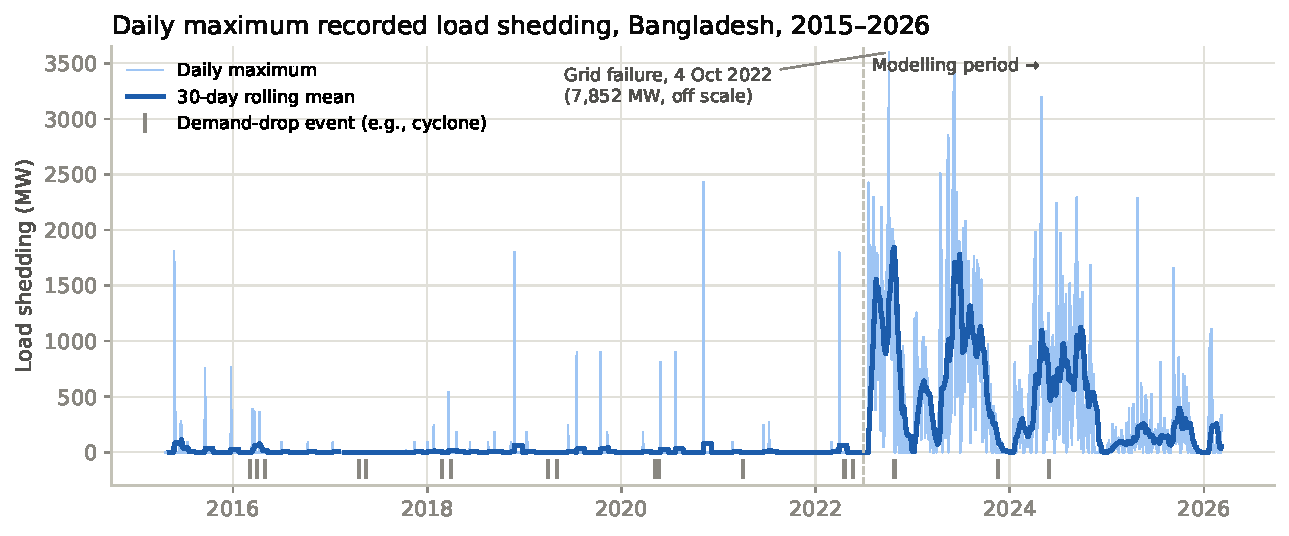
\includegraphics[width=0.82\textwidth]{figures/fig01_daily_load_shedding_trend.pdf}}{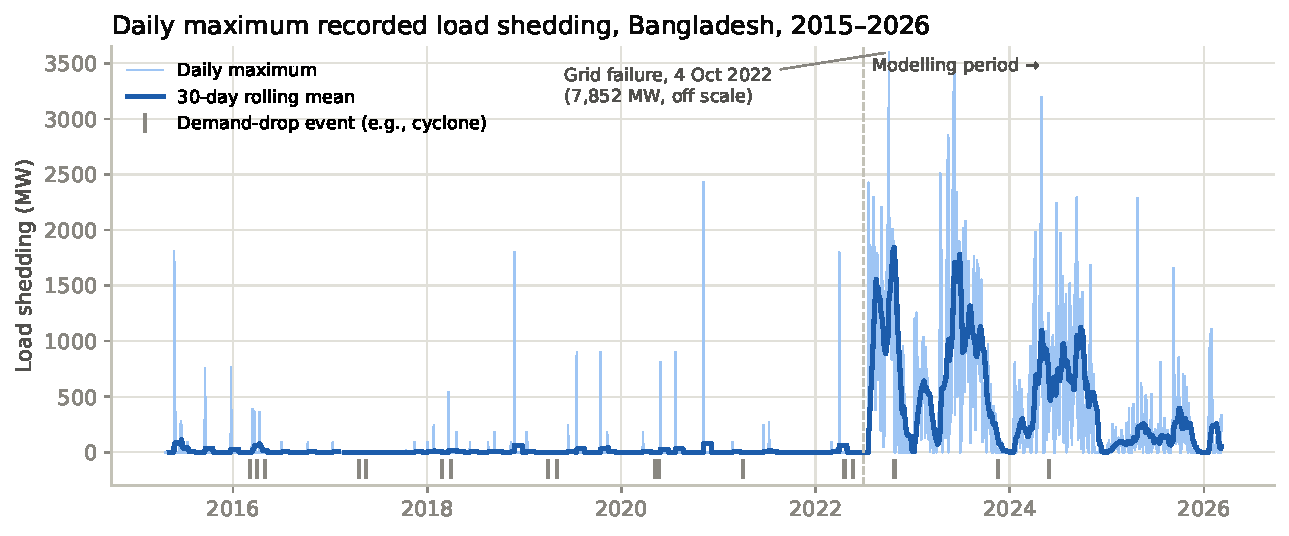
\includegraphics[width=\popw,height=0.8\paperheight,keepaspectratio]{figures/fig01_daily_load_shedding_trend.pdf}}
\caption{Daily maximum national load shedding, 2015--2026 (PGCB data).\enlarge}
\label{fig:trend}
\end{figure*}

\begin{figure}[!t]
\centering
\clickfig{fig:hour}{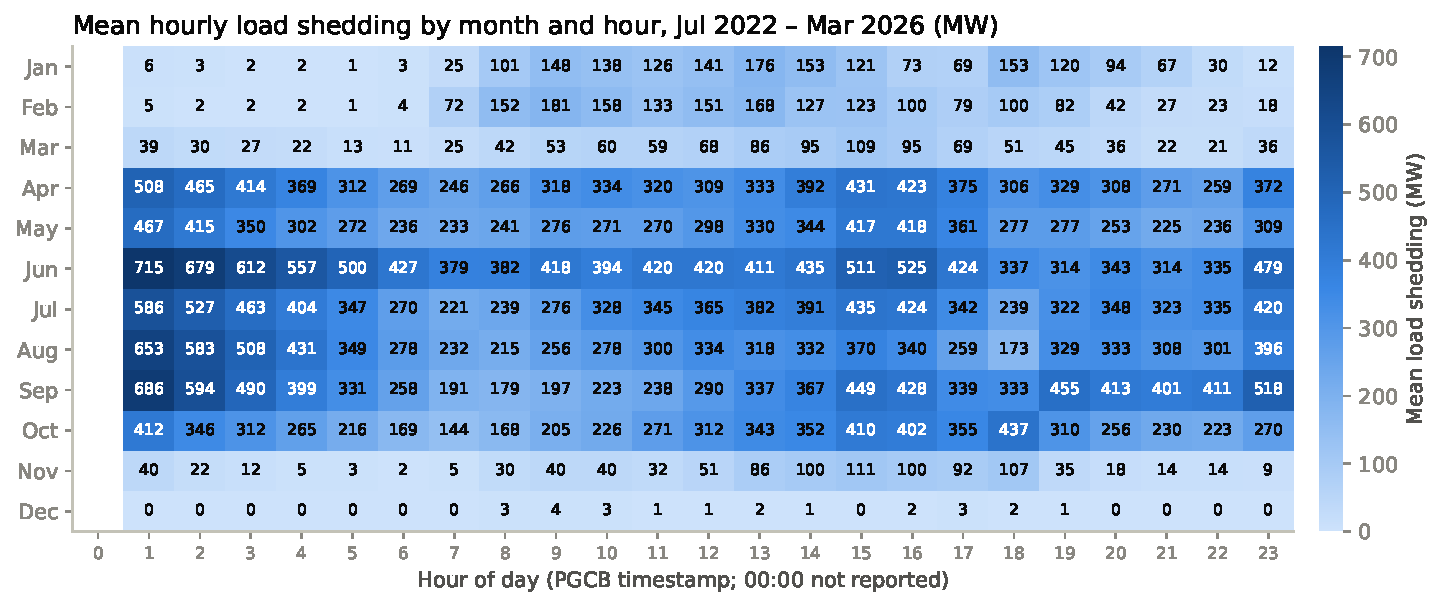
\includegraphics[width=\columnwidth]{figures/fig03_month_hour_heatmap.pdf}}{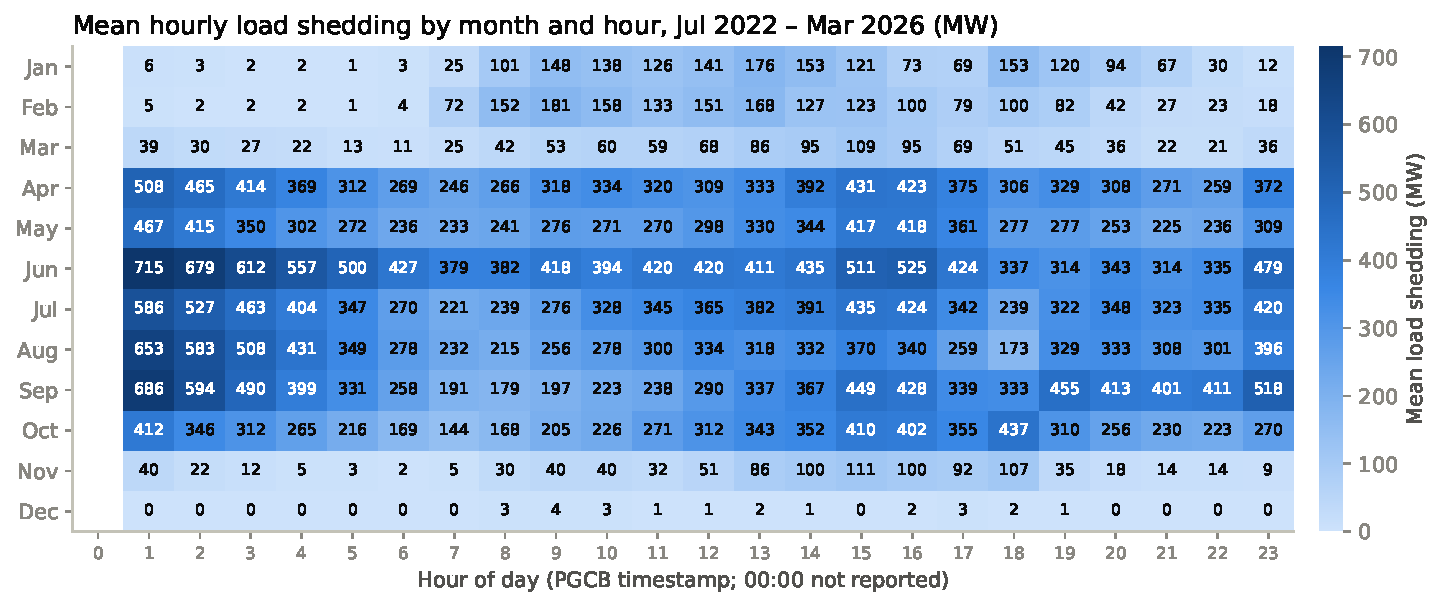
\includegraphics[width=\popw,height=0.8\paperheight,keepaspectratio]{figures/fig03_month_hour_heatmap.pdf}}
\caption{Mean load shedding by month and hour of day, July 2022 to March 2026.\enlarge}
\label{fig:hour}
\end{figure}

\subsection{Predictive Performance (RQ4)}
On the 432-day test period, XGBoost achieved the highest PR-AUC (0.832) and accuracy (0.810) among all models, compared with 0.608 and 0.785 for persistence (Table~\ref{tab:test}; Fig.~\ref{fig:prroc}). Persistence was correct on none of the 93 transition days, whereas XGBoost was correct on 37.6\%; the seasonal naive rule reached 48.4\% on transition days but only 0.609 overall accuracy. The PR-AUC gain over persistence was 0.224 (95\% CI 0.164 to 0.282), while the accuracy gain was 0.026 (95\% CI $-0.014$ to 0.060; McNemar $p = 0.193$, with 35 days on which only the model was correct and 24 on which only persistence was correct) (Table~\ref{tab:sig}). For next-day energy, the LightGBM regressor had a mean absolute error of 757~MWh against 710~MWh for persistence.

\begin{table}[!t]
\caption{Test Performance, January 2025 to March 2026 ($n = 432$)}
\label{tab:test}
\centering
\footnotesize
\begin{tabular}{@{}lccccc@{}}
\toprule
Model & PR-AUC & ROC-AUC & F1 & Acc. & Trans. \\
\midrule
Persistence & 0.608 & 0.768 & 0.707 & 0.785 & 0.0\% \\
Seasonal naive & 0.414 & 0.578 & 0.464 & 0.609 & 48.4\% \\
Seven-day rate & 0.609 & 0.750 & 0.558 & 0.692 & 34.4\% \\
LR & 0.800 & 0.862 & 0.706 & 0.771 & 39.8\% \\
RF & 0.819 & 0.886 & \textbf{0.751} & 0.778 & 38.7\% \\
XGBoost (selected) & \textbf{0.832} & \textbf{0.893} & 0.725 & \textbf{0.810} & 37.6\% \\
LightGBM & 0.812 & 0.883 & 0.715 & 0.748 & 38.7\% \\
\bottomrule
\multicolumn{6}{@{}p{8.3cm}@{}}{\scriptsize Acc.\ = accuracy; Trans.\ = accuracy on the 93 transition days.}
\end{tabular}
\end{table}

\begin{table}[!t]
\caption{Difference Between XGBoost and Persistence on the Test Period}
\label{tab:sig}
\centering
\footnotesize
\begin{tabular}{@{}lccc@{}}
\toprule
Metric & Difference & 95\% CI & Significant \\
\midrule
PR-AUC & $+0.224$ & 0.164 to 0.282 & Yes \\
Transition accuracy & $+0.376$ & 0.304 to 0.446 & Yes \\
Accuracy & $+0.026$ & $-0.014$ to 0.060 & No ($p = 0.193$) \\
F1 & $+0.018$ & $-0.044$ to 0.073 & No \\
\bottomrule
\end{tabular}
\end{table}

\begin{figure}[!t]
\centering
\clickfig{fig:prroc}{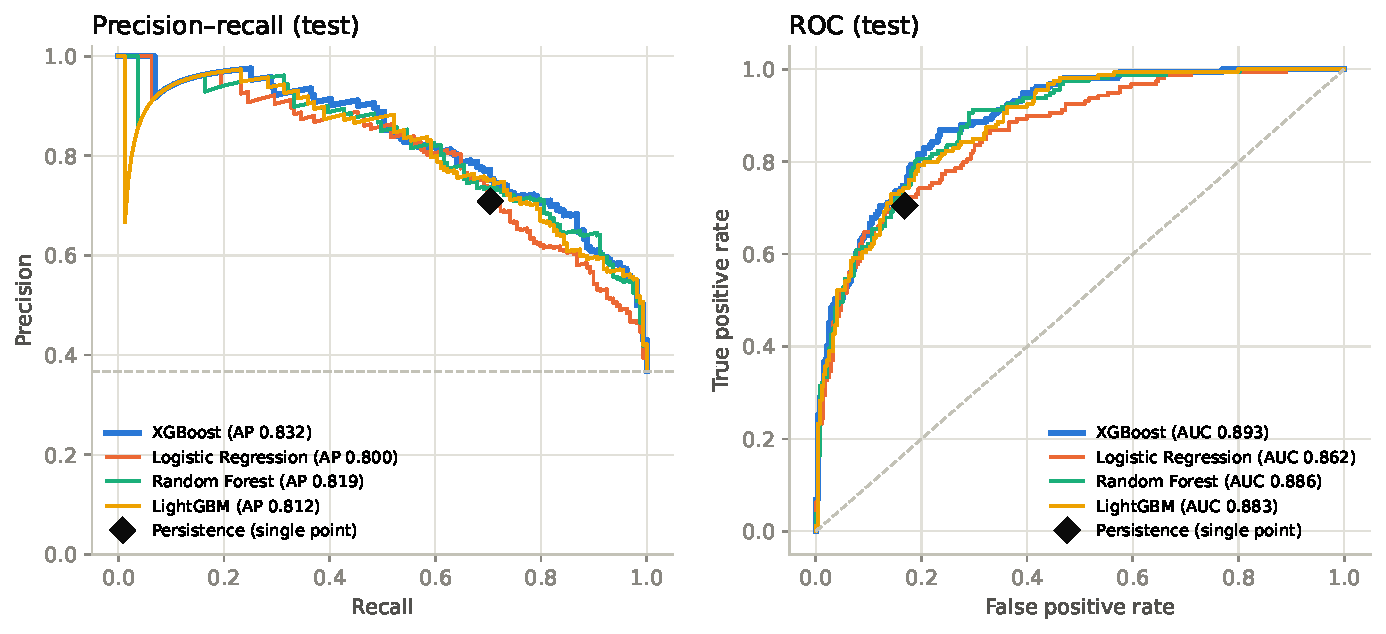
\includegraphics[width=\columnwidth]{figures/fig08_test_pr_roc.pdf}}{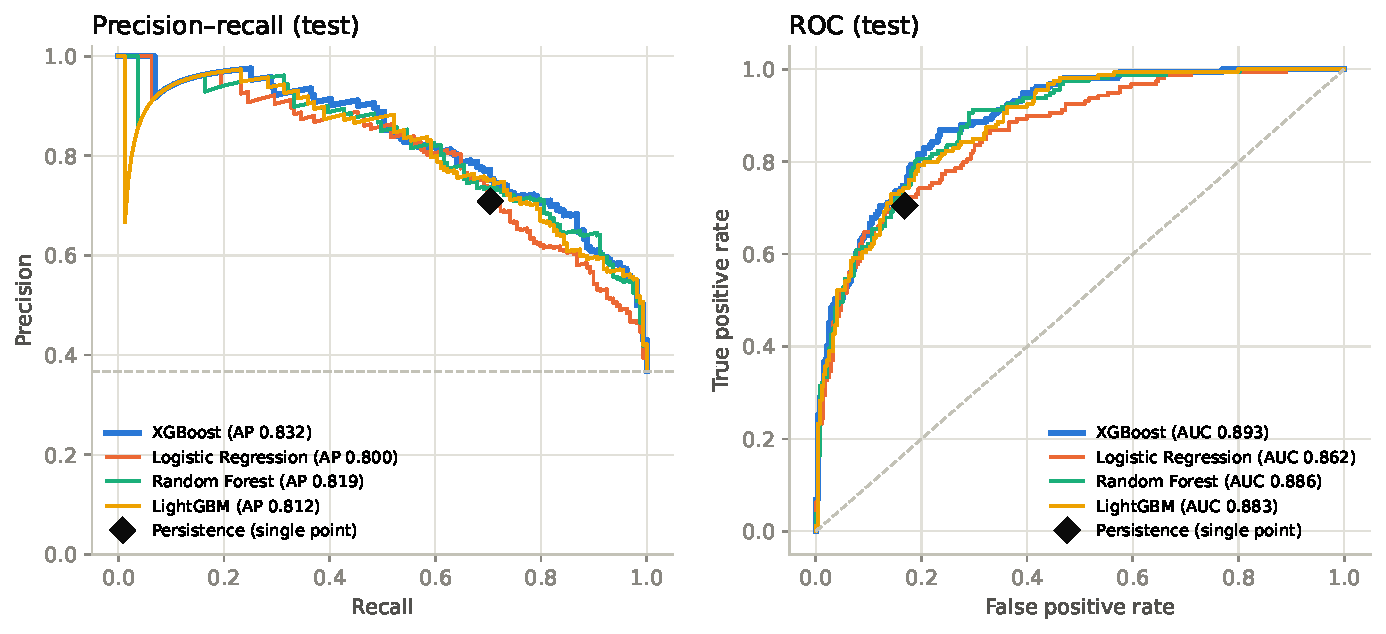
\includegraphics[width=\popw,height=0.8\paperheight,keepaspectratio]{figures/fig08_test_pr_roc.pdf}}
\caption{Precision--recall and receiver operating characteristic curves on the test period.\enlarge}
\label{fig:prroc}
\end{figure}

In robustness checks, the F1 score of the model fell below that of persistence at the 300~MW and 500~MW thresholds (0.609 versus 0.636 and 0.303 versus 0.440). Removing load-shedding history reduced PR-AUC by 0.058, and removing next-day temperature reduced it by 0.005. Five random seeds gave a PR-AUC of $0.828 \pm 0.002$. With misses weighted five times as heavily as false alarms ($k = 5$), the cost-optimal threshold of 0.18 gave 97\% recall and a 48\% lower cost than persistence.

\subsection{Drivers of Risk (RQ2)}
In the full model, load-shedding history accounted for 47.7\% of the mean absolute SHAP value, followed by demand and generation (14.9\%), fuel mix (14.4\%) and calendar (11.3\%) (Table~\ref{tab:shap}). The structural model without history reached a test PR-AUC of 0.775, and its leading feature was the peak demand--generation gap (Fig.~\ref{fig:beeswarm}). Risk increased when next-day maximum temperature exceeded about 32.5~\textdegree C, peak demand exceeded about 12,800~MW (levelling off near 13,800~MW) and the peak gap exceeded about 100~MW (Fig.~\ref{fig:dependence}). An interaction between fuel limitation and heat was not supported.

\begin{table}[!t]
\caption{Share of Mean Absolute SHAP Value by Feature Group (\%)}
\label{tab:shap}
\centering
\footnotesize
\begin{tabular}{@{}lcc@{}}
\toprule
Group & Full model & Structural model \\
\midrule
Load-shedding history & 47.7 & -- \\
Demand and generation & 14.9 & 49.4 \\
Fuel mix & 14.4 & 21.5 \\
Calendar & 11.3 & 15.9 \\
Temperature, day $t+1$ & 7.7 & 5.7 \\
Temperature, day $t$ & 2.3 & 2.8 \\
Supply constraints & 1.7 & 4.7 \\
\bottomrule
\end{tabular}
\end{table}

\begin{figure}[!t]
\centering
\clickfig{fig:beeswarm}{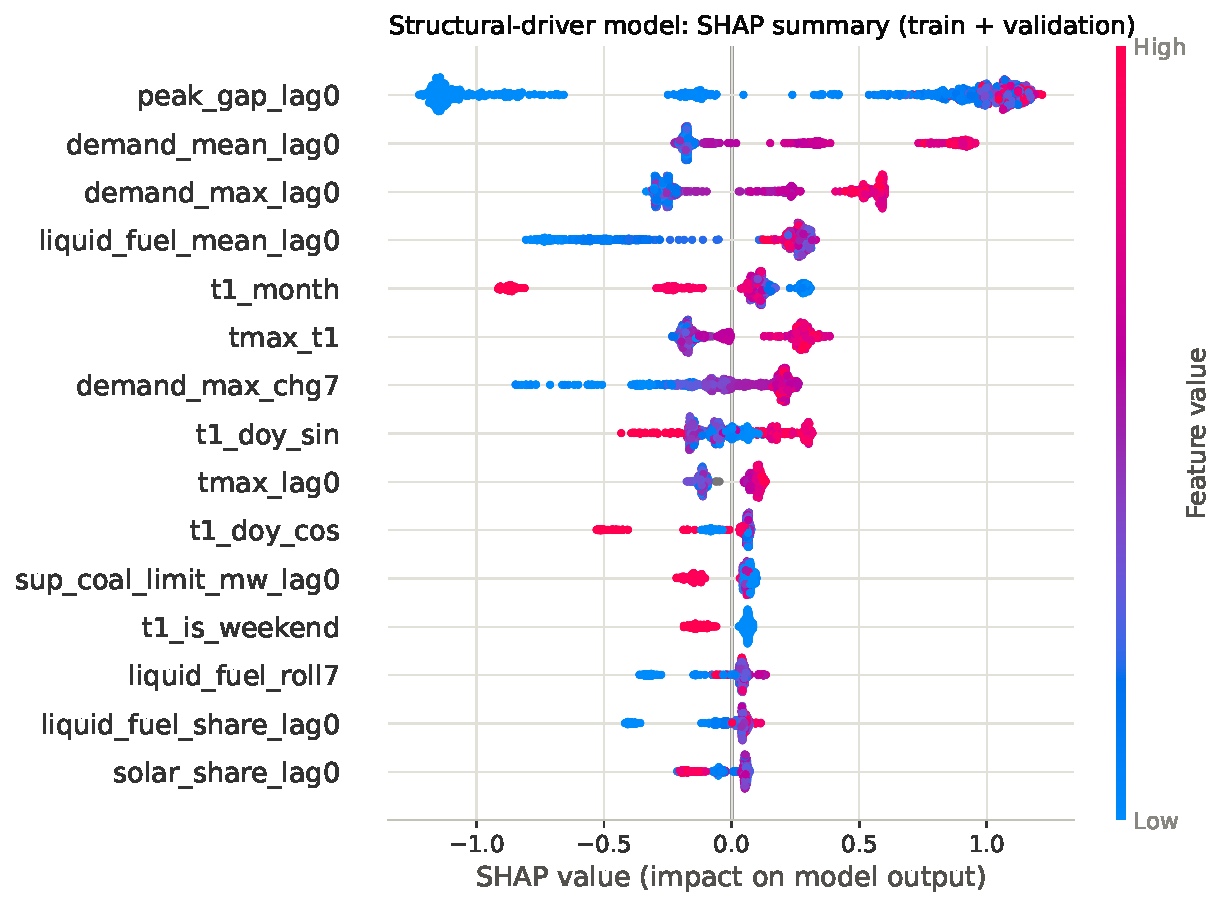
\includegraphics[width=\columnwidth]{figures/fig13_shap_structural_beeswarm.pdf}}{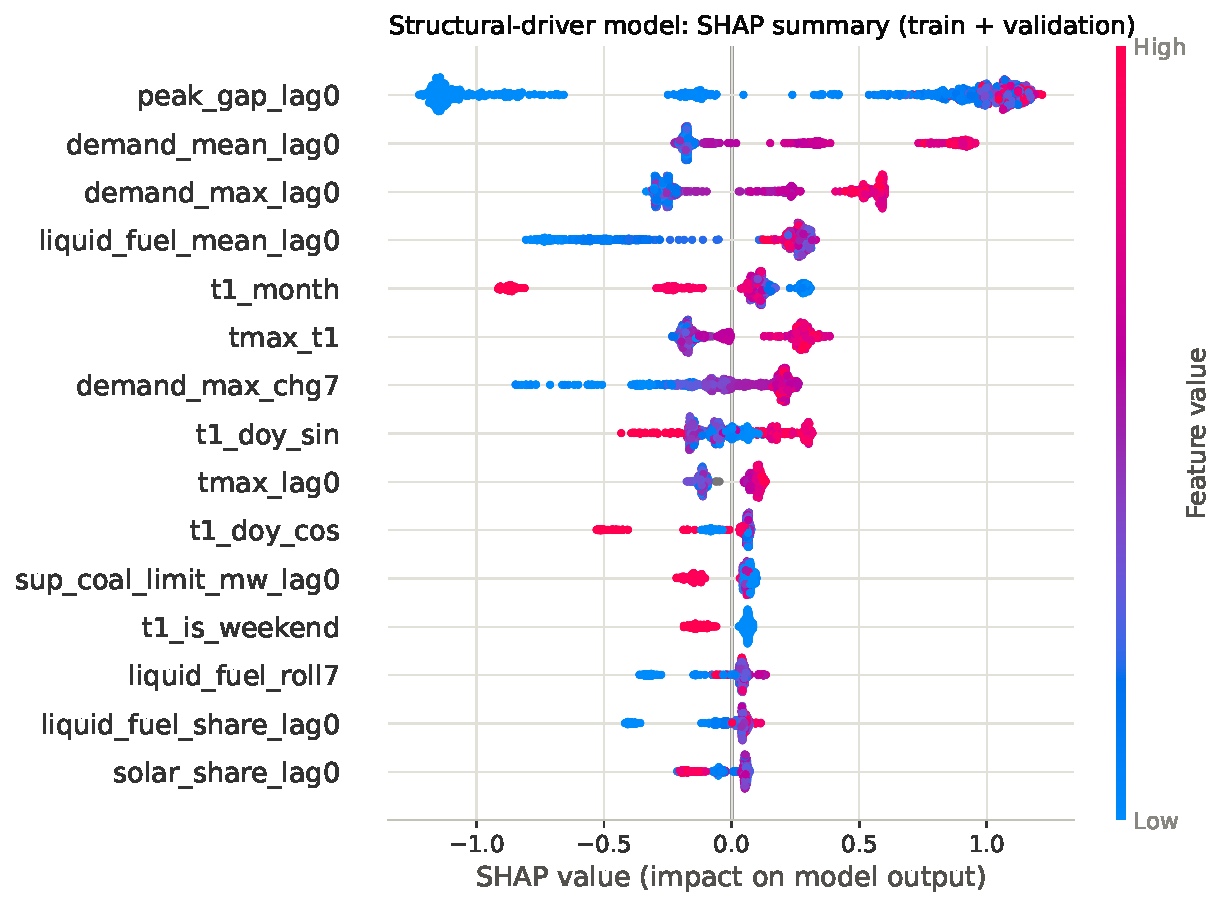
\includegraphics[width=\popw,height=0.8\paperheight,keepaspectratio]{figures/fig13_shap_structural_beeswarm.pdf}}
\caption{SHAP values of the structural model, trained without load-shedding history.\enlarge}
\label{fig:beeswarm}
\end{figure}

\begin{figure*}[!t]
\centering
\clickfig{fig:dependence}{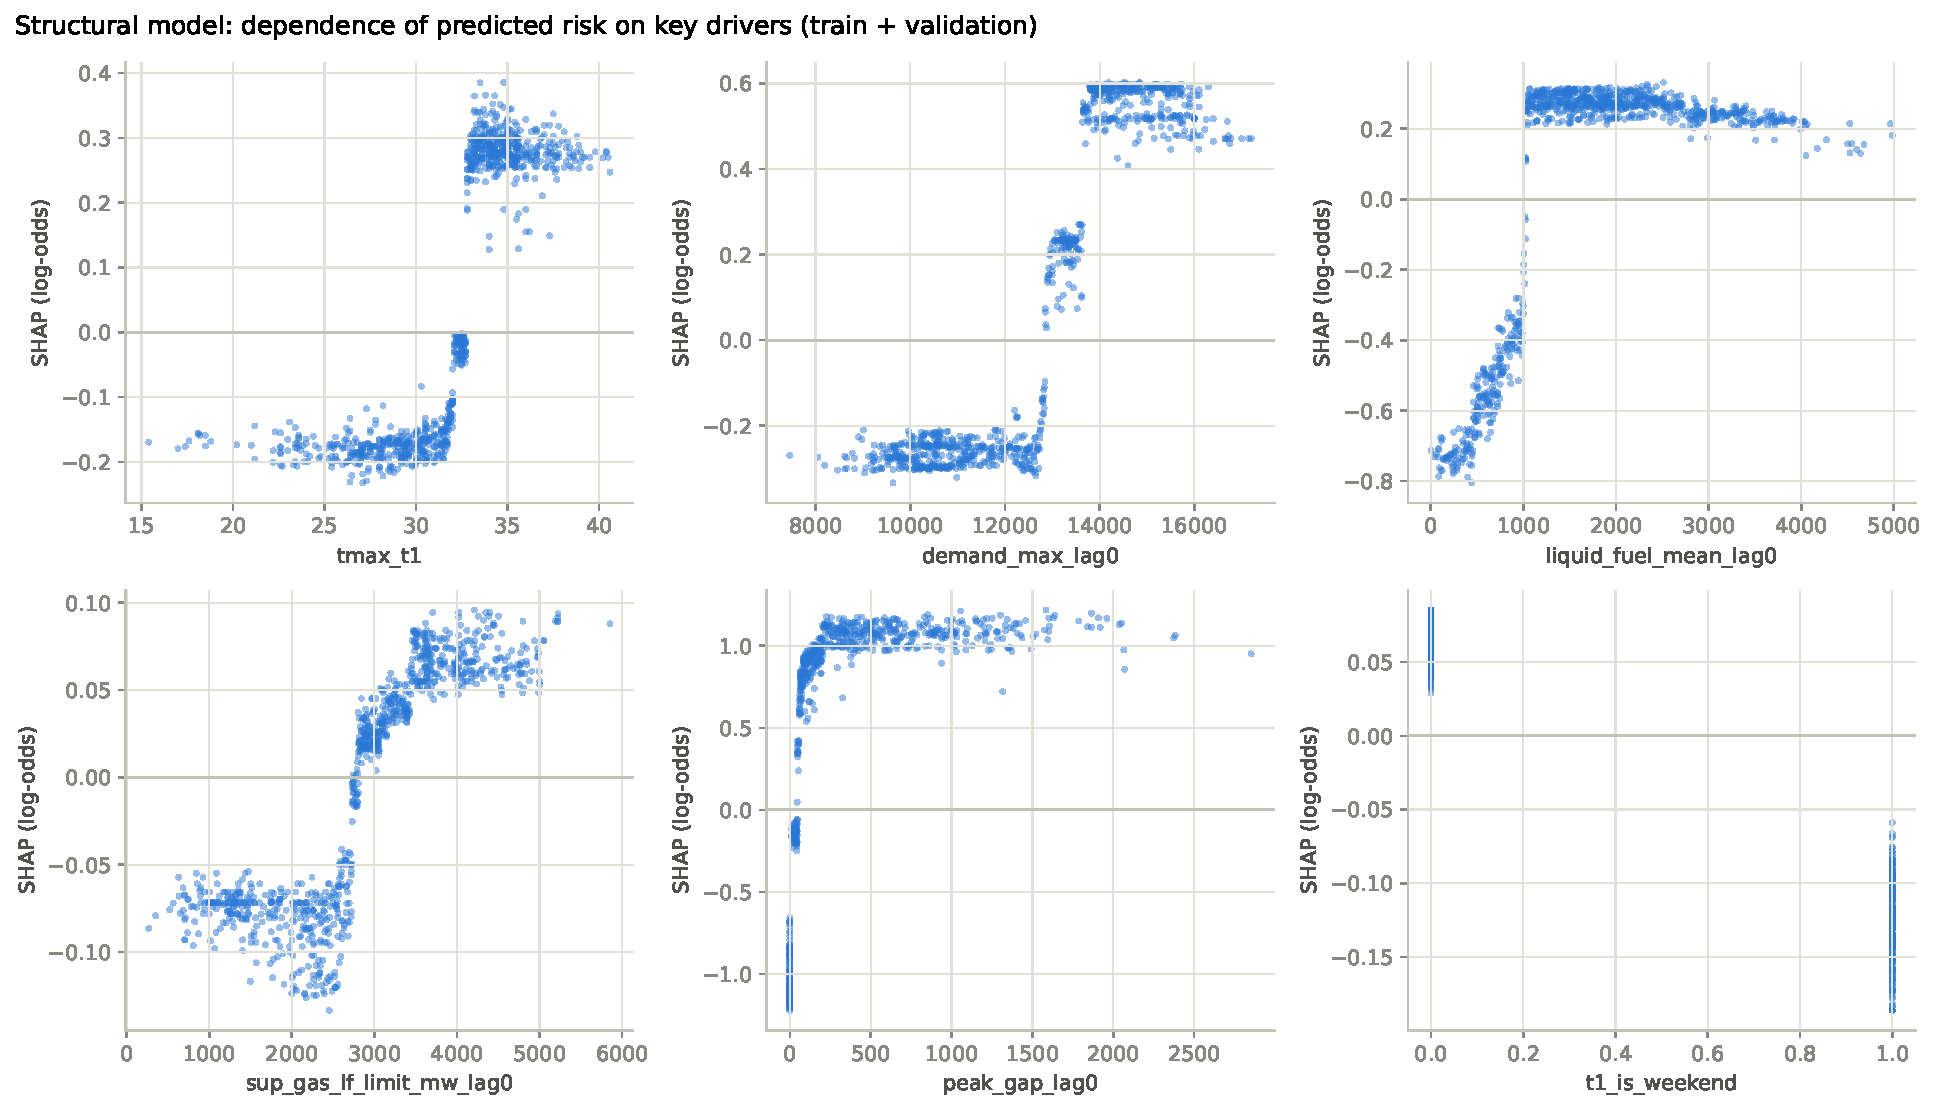
\includegraphics[width=0.78\textwidth]{figures/fig14_shap_dependence.pdf}}{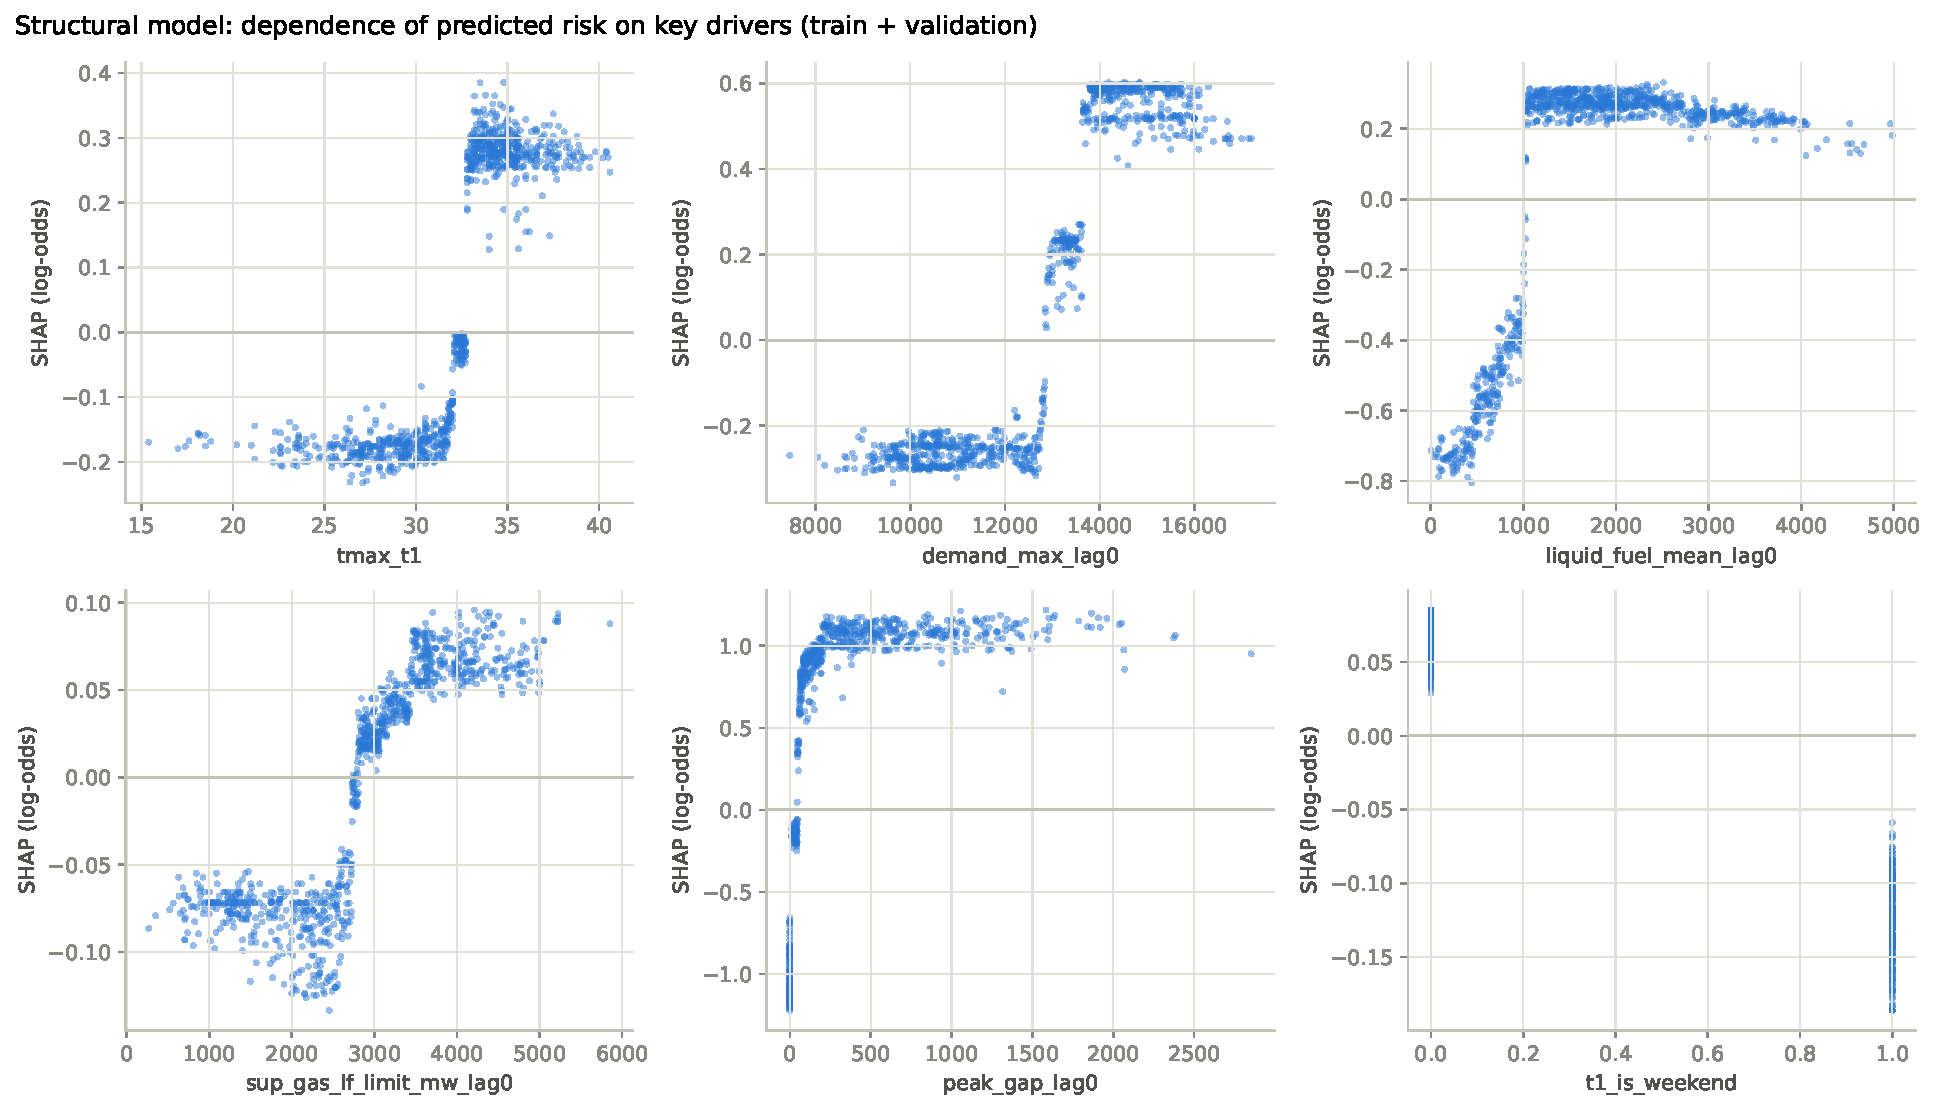
\includegraphics[width=\popw,height=0.8\paperheight,keepaspectratio]{figures/fig14_shap_dependence.pdf}}
\caption{SHAP dependence of predicted risk on six drivers in the structural model: next-day maximum temperature, peak demand, liquid-fuel generation, gas and liquid-fuel limitation, peak demand--generation gap and weekend (training and validation data).\enlarge}
\label{fig:dependence}
\end{figure*}

\subsection{Transfer to a Second Crisis (RQ4)}
Positive days made up 19.6\% of 2025 and 49.1\% of January to August 2026 (Table~\ref{tab:twocrisis}). In 2026, the frozen LightGBM model reached an accuracy of 0.893 and a PR-AUC of 0.925, compared with 0.860 and 0.807 for persistence (McNemar $p = 0.119$; 11 days on which only the model was correct and 4 on which only persistence was correct). In 2025, its PR-AUC was higher (0.628 versus 0.403) but its accuracy was lower (0.798 versus 0.829), and it caught 18 of 31 episode onsets. The monthly retrained model reached an accuracy of 0.860 in 2026. Of four episode onsets in 2026, the frozen model warned on 2 April (probability 0.481 against a threshold of 0.48) and 1 June (0.671), and missed 20 January and 5 May (Fig.~\ref{fig:crisis2026}).

\begin{table}[!t]
\caption{Two-Crisis Test on the BPDB National Series}
\label{tab:twocrisis}
\centering
\footnotesize
\begin{tabular}{@{}llcccc@{}}
\toprule
Test & Model & PR-AUC & Acc. & F1 & Onsets \\
\midrule
\multirow{3}{*}{\shortstack[l]{2025\\($n=362$)}} & Persistence & 0.403 & 0.829 & 0.563 & 0/31 \\
 & Frozen & 0.628 & 0.798 & 0.610 & 18/31 \\
 & Monthly & 0.596 & 0.804 & 0.523 & 5/31 \\
\midrule
\multirow{3}{*}{\shortstack[l]{2026\\($n=214$)}} & Persistence & 0.807 & 0.860 & 0.856 & 0/16 \\
 & Frozen & 0.925 & 0.893 & 0.891 & 8/16 \\
 & Monthly & 0.927 & 0.860 & 0.851 & 4/16 \\
\bottomrule
\multicolumn{6}{@{}p{8.3cm}@{}}{\scriptsize Frozen and Monthly are LightGBM models trained to December 2024 and retrained every month, respectively.}
\end{tabular}
\end{table}

\begin{figure*}[!t]
\centering
\clickfig{fig:crisis2026}{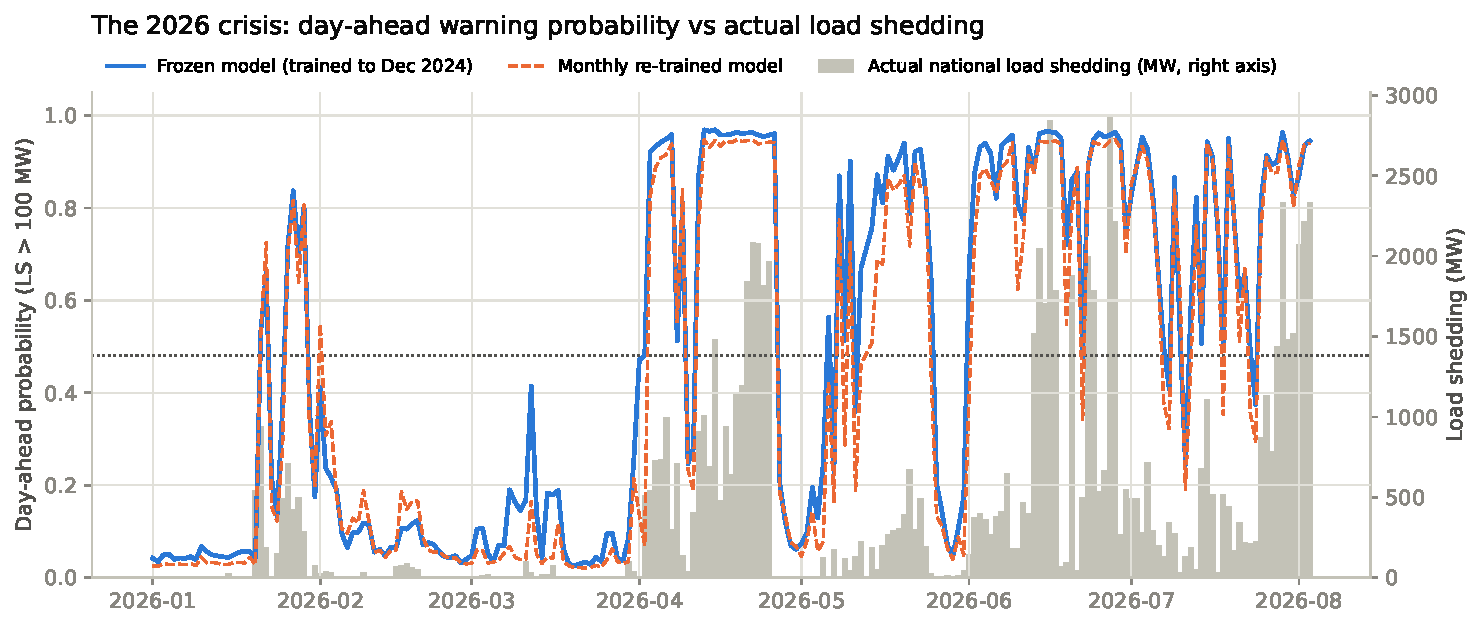
\includegraphics[width=0.82\textwidth]{figures/fig40_2026_crisis_timeline.pdf}}{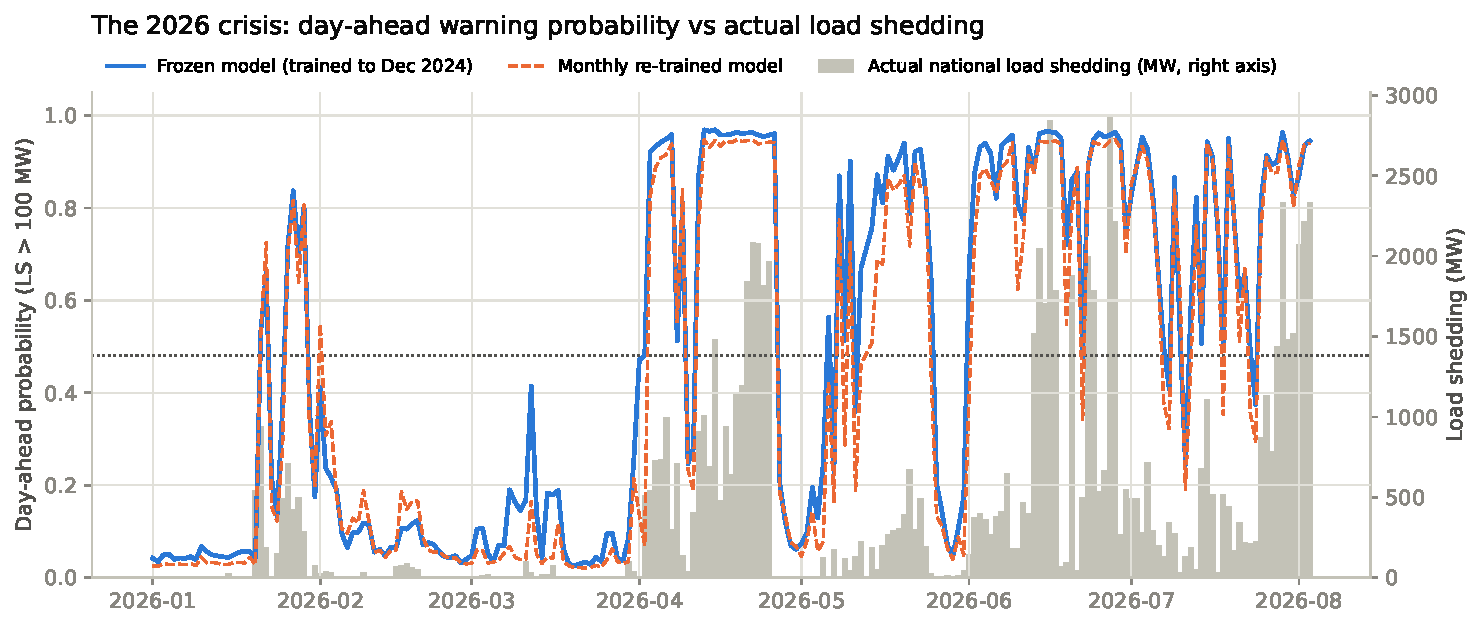
\includegraphics[width=\popw,height=0.8\paperheight,keepaspectratio]{figures/fig40_2026_crisis_timeline.pdf}}
\caption{Day-ahead warning probability of the frozen and monthly retrained models against actual national load shedding, January to August 2026. The dotted line marks the decision threshold of 0.48.\enlarge}
\label{fig:crisis2026}
\end{figure*}

\subsection{Regional Distribution (RQ3)}
In the crisis period (July 2022 to December 2024), Mymensingh accounted for 8.4\% of demand and 27.5\% of load shedding ($R_z = 3.27$), whereas Dhaka (0.57), Chattogram (0.44) and Barishal (0.20) received less than their demand share (Table~\ref{tab:zones}). The Gini coefficient \eqref{eq:gini} was 0.36 in the crisis period and 0.38 afterwards; by year it was highest in 2025 (0.51), when national intensity was lowest (0.5\%). On days with 1 to 100~MW of national shedding ($n = 306$), Mymensingh shed load on 76\% of days and carried 65.4\% of national shedding; above 1,500~MW ($n = 37$) its share was 14.0\% (Fig.~\ref{fig:order}). The zone premium was $+0.48$ log-odds for Mymensingh and $-0.42$ for Barishal (Fig.~\ref{fig:premium}). The zone-level model reached a ROC-AUC of 0.884 in 2025 and 0.905 in 2026, with accuracy equal to persistence in 2025 (0.885) and slightly higher in 2026 (0.841 versus 0.829).

\begin{table}[!t]
\caption{Share of Demand and Load Shedding by Zone}
\label{tab:zones}
\centering
\footnotesize
\begin{tabular}{@{}lcccc@{}}
\toprule
Zone & Demand (\%) & Shedding (\%) & $R_z$ & $R_z$, 2025--26 \\
\midrule
Mymensingh & 8.4 & 27.5 & 3.27 & 3.74 \\
Rangpur & 6.7 & 10.8 & 1.61 & 1.38 \\
Cumilla & 9.4 & 13.3 & 1.41 & 1.06 \\
Sylhet & 4.0 & 5.5 & 1.38 & 1.30 \\
Rajshahi & 10.4 & 8.7 & 0.83 & 0.80 \\
Khulna & 12.1 & 8.7 & 0.72 & 1.04 \\
Dhaka & 36.1 & 20.6 & 0.57 & 0.45 \\
Chattogram & 10.0 & 4.4 & 0.44 & 0.48 \\
Barishal & 3.0 & 0.6 & 0.20 & 0.85 \\
\bottomrule
\multicolumn{5}{@{}p{8.3cm}@{}}{\scriptsize Shares and $R_z$ \eqref{eq:ratio} refer to July 2022 to December 2024; the last column covers January 2025 to August 2026.}
\end{tabular}
\end{table}

\begin{figure}[!t]
\centering
\clickfig{fig:order}{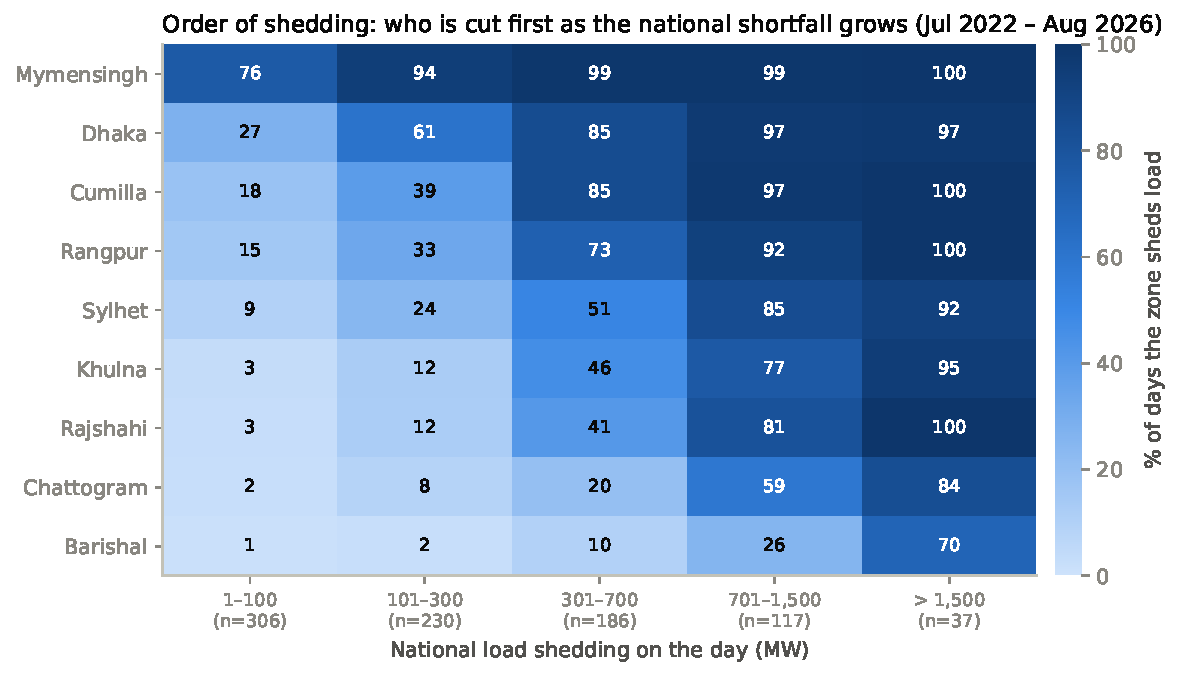
\includegraphics[width=\columnwidth]{figures/fig42_order_of_shedding.pdf}}{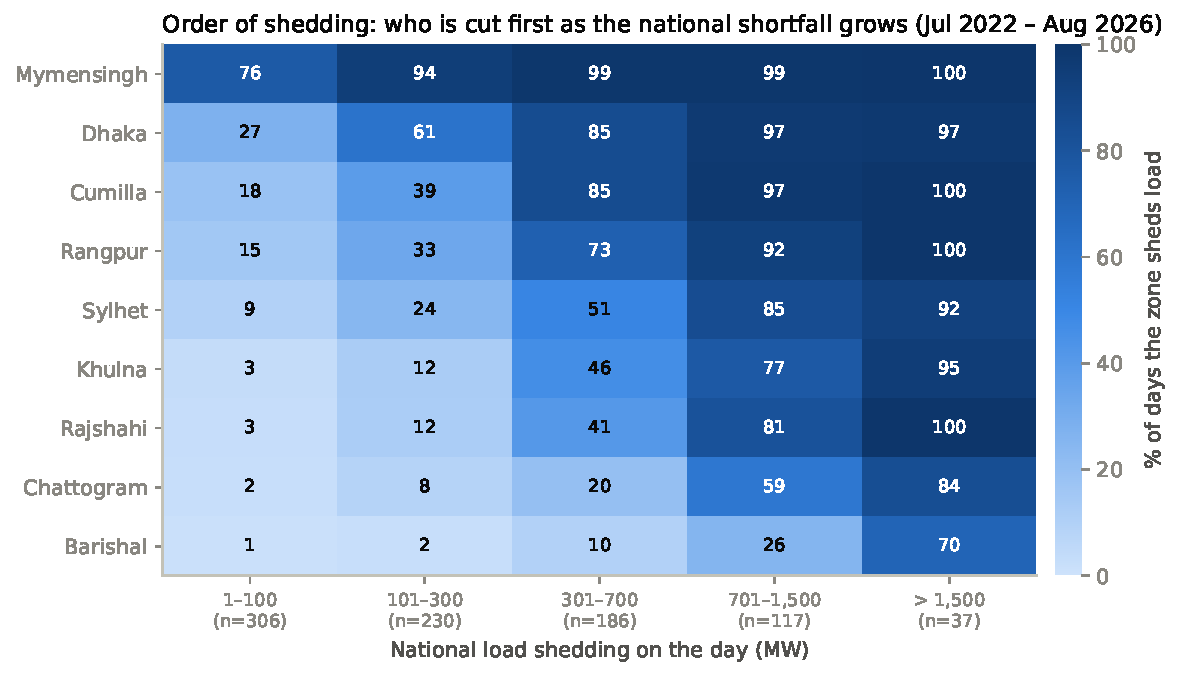
\includegraphics[width=\popw,height=0.8\paperheight,keepaspectratio]{figures/fig42_order_of_shedding.pdf}}
\caption{Share of days on which each zone shed load, by national shortfall, July 2022 to August 2026.\enlarge}
\label{fig:order}
\end{figure}

\begin{figure*}[!t]
\centering
\clickfig{fig:premium}{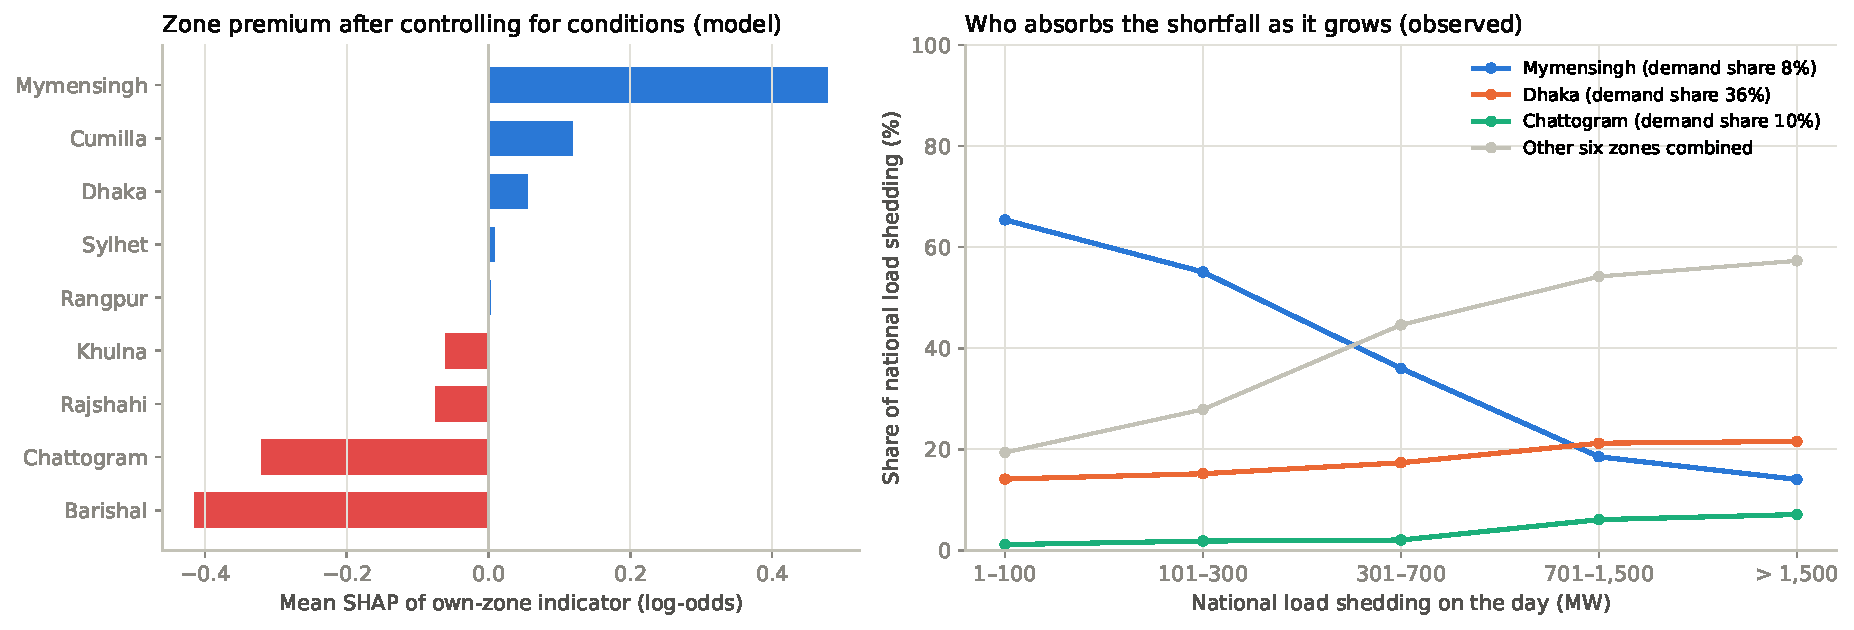
\includegraphics[width=0.82\textwidth]{figures/fig43_zone_premium_and_share.pdf}}{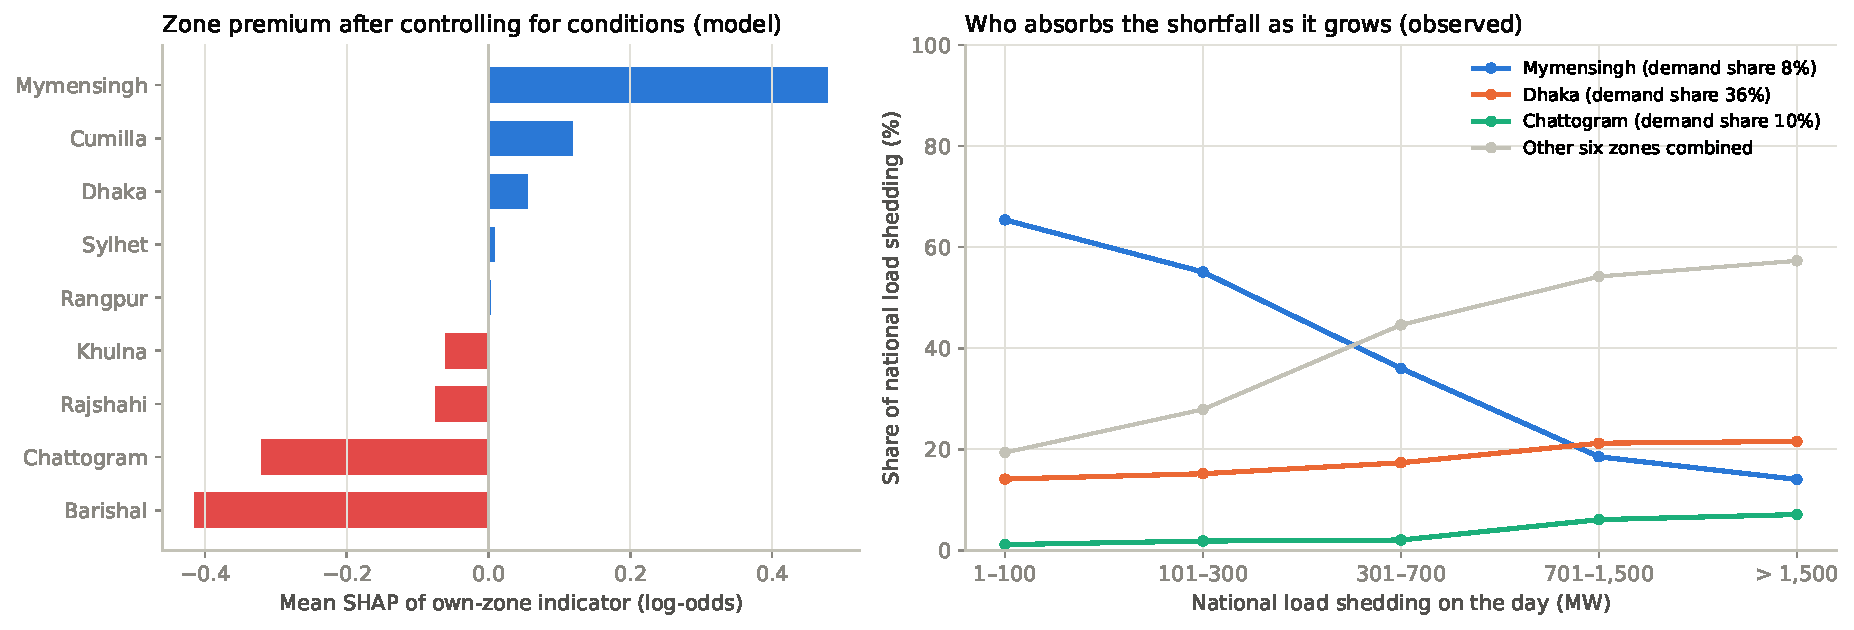
\includegraphics[width=\popw,height=0.8\paperheight,keepaspectratio]{figures/fig43_zone_premium_and_share.pdf}}
\caption{Zone premium from the panel model (left) and observed share of national load shedding by national shortfall (right).\enlarge}
\label{fig:premium}
\end{figure*}

% ===========================================================================
\section{Discussion}\label{sec:discussion}
% ===========================================================================
\subsection{Main Findings}
Day-ahead load shedding in Bangladesh is partly predictable. Gradient boosting ranks risky days clearly better than persistence and recovers more than a third of the days on which the situation changes, which persistence cannot do by construction. On the simpler question of whether tomorrow will be a load-shedding day, however, its advantage is small and not statistically significant, because load shedding runs in long episodes that persistence already captures. The null hypothesis of equal accuracy could therefore not be rejected, whereas that of equal ranking performance was rejected.

\subsection{Comparison With Earlier Studies}
Unlike forecasting work on Bangladesh that predicts demand~\cite{akhter2024}, this study predicts the shortfall itself, and unlike control-oriented studies~\cite{zhou2024,gain2025} it works with observed national records rather than simulations. Earlier load-shedding classifiers~\cite{rahman2016,arifuzzaman2026,akinola2024} did not report a persistence baseline; our comparison suggests that headline classification scores should be read against how strongly load shedding persists from day to day. As in outage prediction~\cite{wanik2015,taylor2023}, gradient-boosted trees performed well on tabular inputs. The equity findings extend fairness analysis of planned schemes~\cite{heylen2018} to the shedding that customers actually received, and they agree with press reports that Mymensingh bears a disproportionate share~\cite{dailystar2026}. A student poster based on night-time lights reported that Rajshahi and Rangpur fared worse than urban divisions~\cite{mitchell2026}; our zone data agree for Rangpur but not for Rajshahi, which may reflect the difference between measuring electricity use and reported shedding.

\subsection{Unexpected Findings}
Three results were not anticipated. First, the frozen model outperformed monthly retraining in 2026. A plausible explanation is that retraining on the calm year taught the model that heat and high demand did not lead to shedding, making it slower to react when the crisis returned; this crisis-memory effect rests on a single crisis and should be treated as a hypothesis. Second, inequality was highest in 2025, when total shedding was lowest. The order of shedding explains this: small shortfalls fall mostly on Mymensingh, whereas large shortfalls spread across all zones. Third, supply-constraint features contributed little to SHAP importance despite the fuel crisis, probably because the reported limitations change slowly from day to day and their effect is already reflected in generation and fuel-mix variables.

\subsection{Strengths and Limitations}
Strengths include two independent data sources that agree closely, a leakage-free design with a single use of the test period, comparison with persistence, significance testing and two out-of-sample periods. Several limitations apply. Next-day temperature was taken from observations, which overstates what a real forecast would provide, although removing it changed PR-AUC by only 0.005. Temperature was available only for Dhaka. The regime shift in 2025 reduced test positives to 37\%, and the test periods (432 and 214 days) limit statistical power. SHAP values and the zone premium describe the model and are not causal estimates. Official figures may understate the shedding customers experience. Finally, the model predicts daily national or zonal events and not their timing within a day.

\subsection{Implications}
For grid operators, a daily risk score is most useful when a missed warning is costly: with misses weighted five times as heavily as false alarms, the model reduced the expected cost by 48\% relative to persistence. For regulators, the order of shedding offers a measurable target: rotating shedding on low-shortfall days would spread a burden that now falls mostly on Mymensingh. For modellers, the results caution against retraining only on recent calm periods and argue for always reporting a persistence baseline.

% ===========================================================================
\section{Conclusion}\label{sec:conclusion}
% ===========================================================================
This study developed and evaluated an interpretable day-ahead early-warning model for load shedding in Bangladesh and measured how shedding is distributed across the country. Gradient boosting ranks next-day risk and anticipates turning points better than persistence, although its everyday accuracy gain is small and not statistically significant. A model trained on the 2022--2024 crisis transferred to the 2026 crisis, while monthly retraining on a calm year weakened it. High next-day temperature, high demand and a positive demand--supply gap mark the riskiest days, and small shortfalls fall disproportionately on Mymensingh.

These findings show that public grid data can support both early warning and equity monitoring, provided that models are judged against simple baselines. Future work should use real weather forecasts and zone-level temperature, add fuel-import schedules, predict the hour of shedding, and test rotation rules that share small shortfalls more evenly. Making load shedding predictable and fair is as much a question of transparent data as of generation capacity.

\section*{Acknowledgment}
The authors thank the providers of the public PGCB and BPDB datasets. An AI assistant (Claude, Anthropic) was used to help write analysis code and draft text; the authors checked all results and take full responsibility for the content.

\bibliographystyle{IEEEtran}
\bibliography{refs}
\iffullfigs
\clearpage
\onecolumn
\section*{Full-Size Figures}
Each figure below is the full-page version of a figure in the text. Click the link under a figure to return to it.
\clearpage
\fullfigL{fig:framework}{\resizebox{\textwidth}{!}{\frameworkdiagram}}{Research framework. Shaded boxes are input datasets; outlined blue boxes are the two novel analyses.}
\fullfigL{fig:trend}{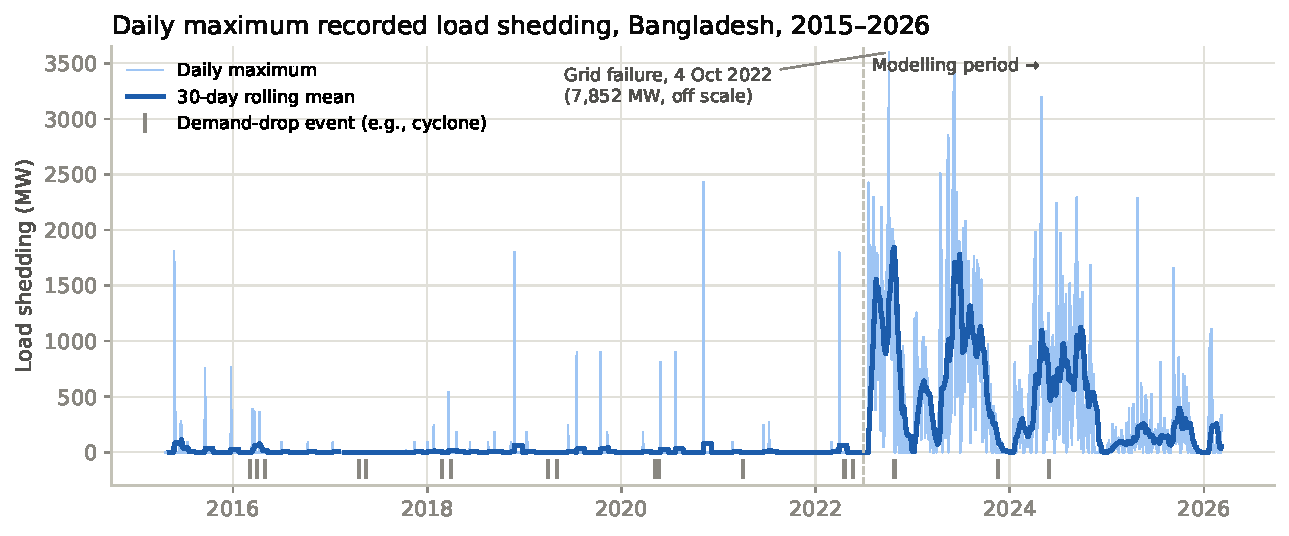
\includegraphics[width=\textwidth,height=0.72\textheight,keepaspectratio]{figures/fig01_daily_load_shedding_trend.pdf}}{Daily maximum national load shedding, 2015--2026 (PGCB data).}
\fullfig{fig:hour}{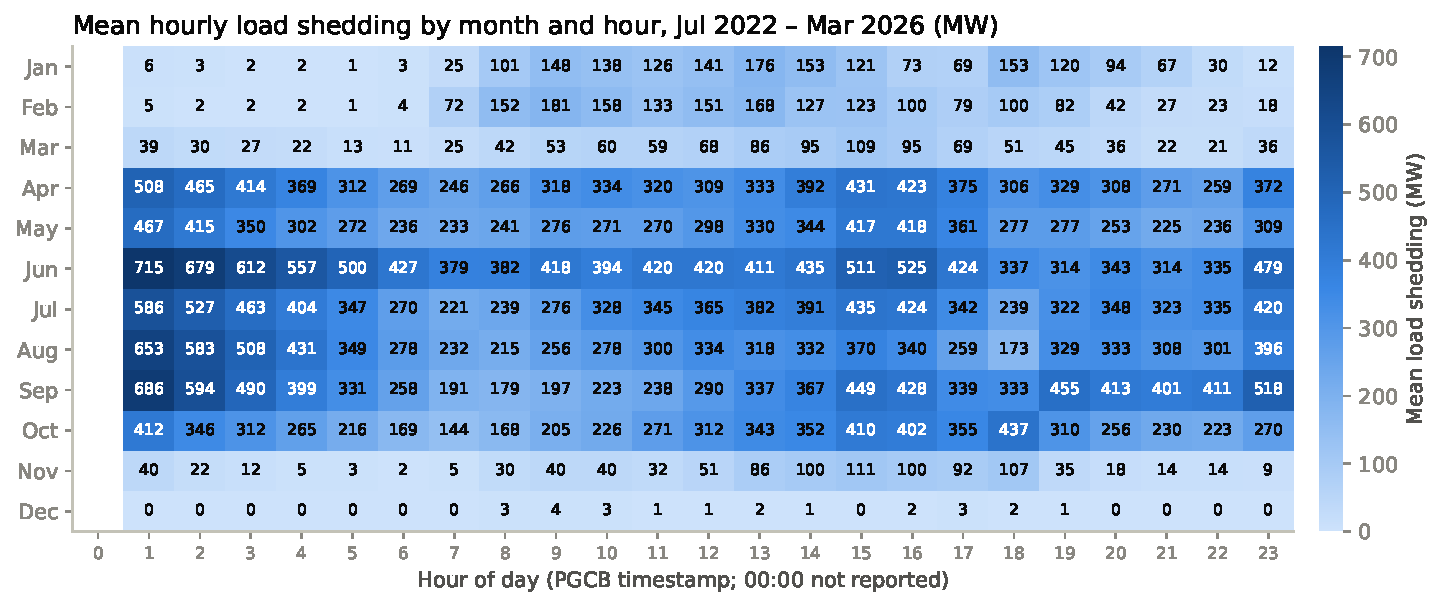
\includegraphics[width=\textwidth,height=0.72\textheight,keepaspectratio]{figures/fig03_month_hour_heatmap.pdf}}{Mean load shedding by month and hour of day, July 2022 to March 2026.}
\fullfig{fig:prroc}{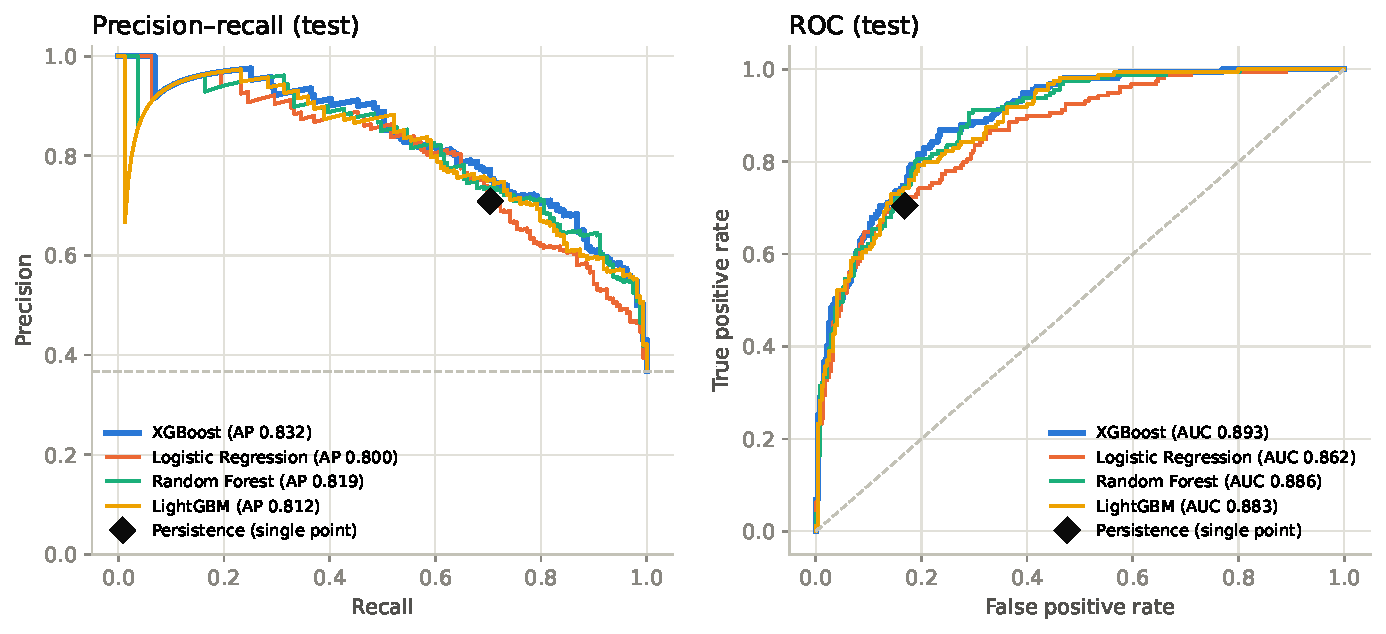
\includegraphics[width=\textwidth,height=0.72\textheight,keepaspectratio]{figures/fig08_test_pr_roc.pdf}}{Precision--recall and receiver operating characteristic curves on the test period.}
\fullfig{fig:beeswarm}{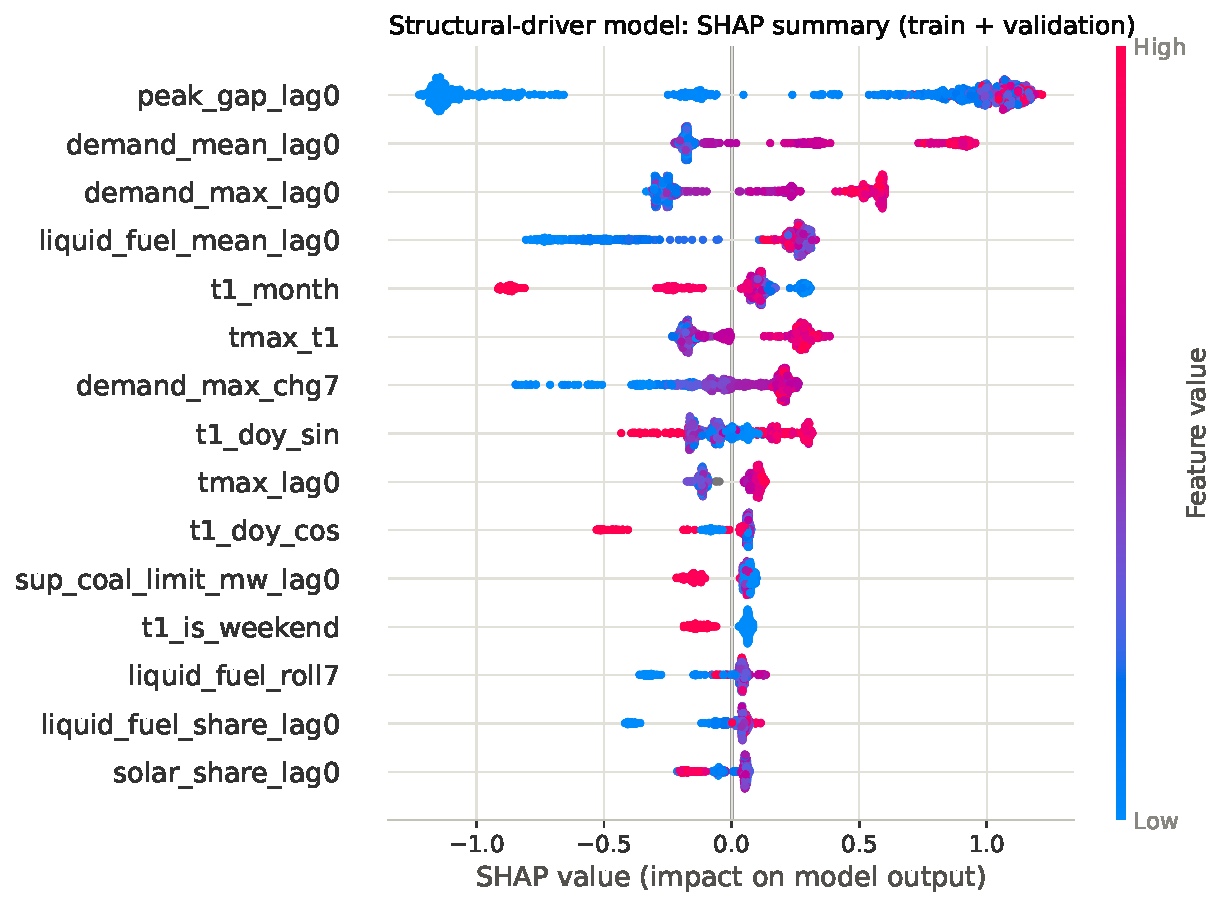
\includegraphics[width=\textwidth,height=0.72\textheight,keepaspectratio]{figures/fig13_shap_structural_beeswarm.pdf}}{SHAP values of the structural model, trained without load-shedding history.}
\fullfigL{fig:dependence}{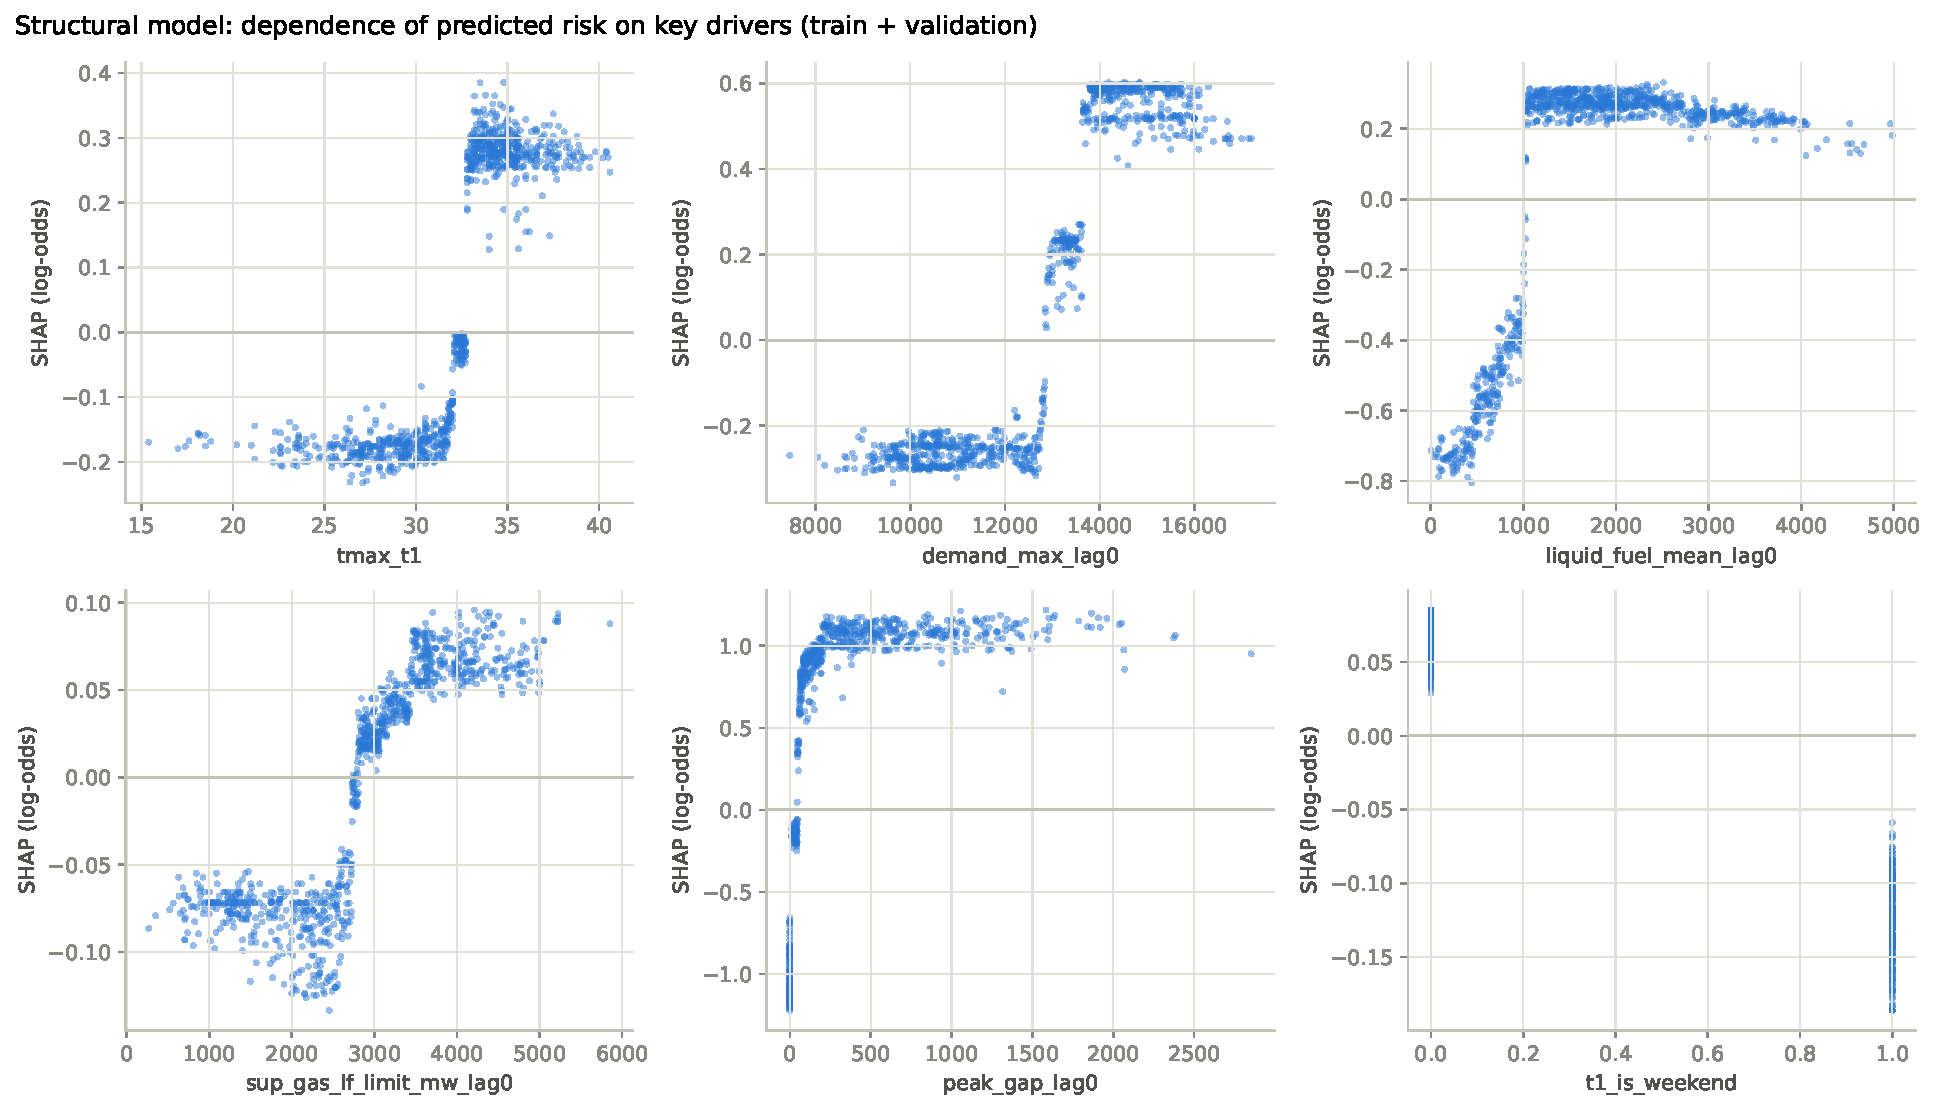
\includegraphics[width=\textwidth,height=0.72\textheight,keepaspectratio]{figures/fig14_shap_dependence.pdf}}{SHAP dependence of predicted risk on six drivers in the structural model: next-day maximum temperature, peak demand, liquid-fuel generation, gas and liquid-fuel limitation, peak demand--generation gap and weekend (training and validation data).}
\fullfigL{fig:crisis2026}{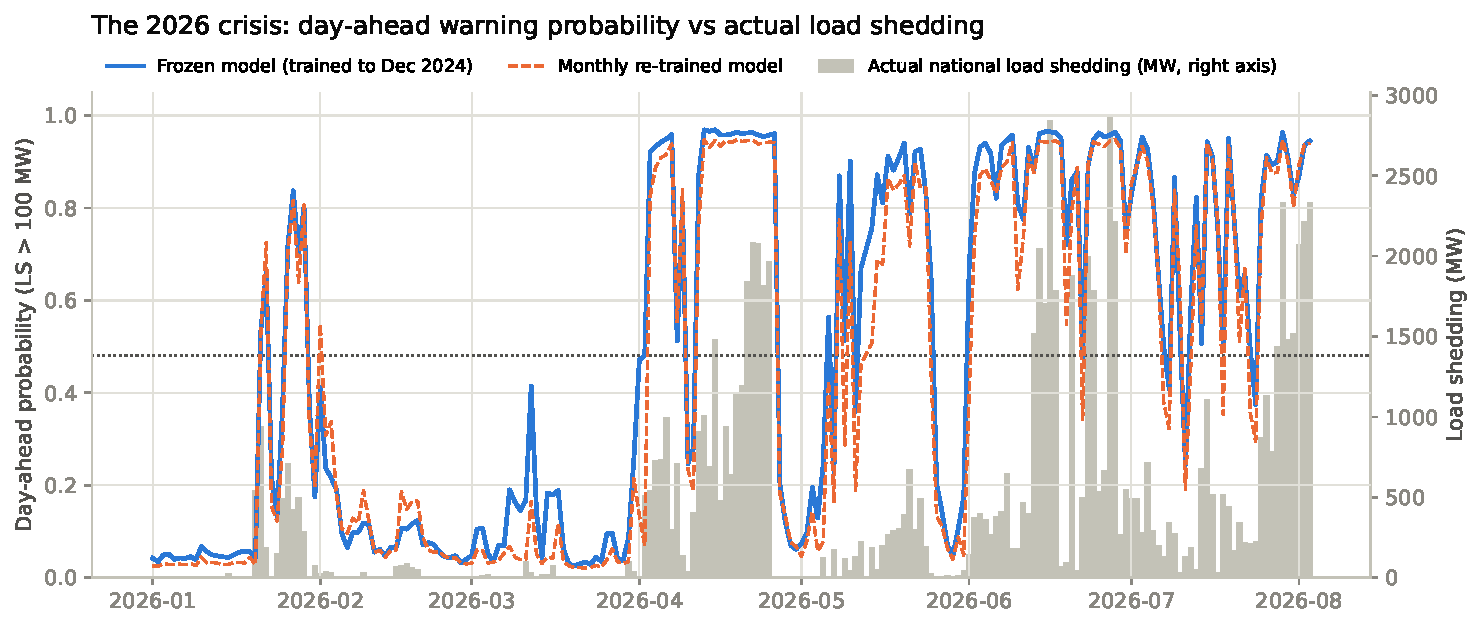
\includegraphics[width=\textwidth,height=0.72\textheight,keepaspectratio]{figures/fig40_2026_crisis_timeline.pdf}}{Day-ahead warning probability of the frozen and monthly retrained models against actual national load shedding, January to August 2026. The dotted line marks the decision threshold of 0.48.}
\fullfig{fig:order}{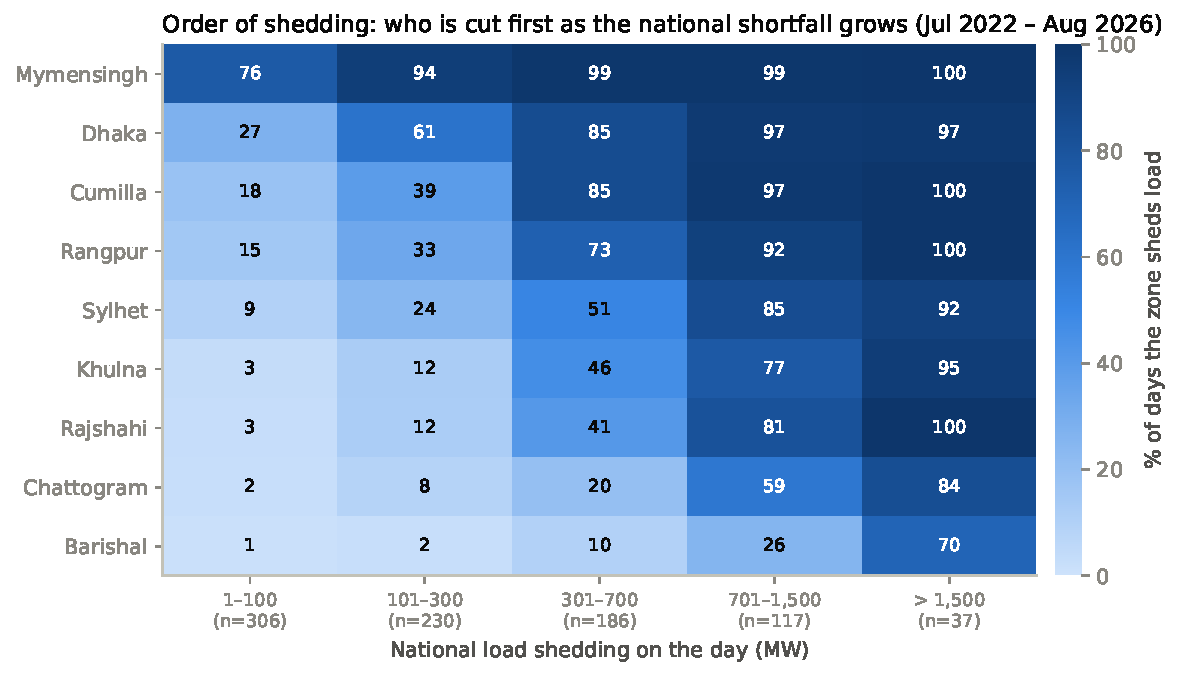
\includegraphics[width=\textwidth,height=0.72\textheight,keepaspectratio]{figures/fig42_order_of_shedding.pdf}}{Share of days on which each zone shed load, by national shortfall, July 2022 to August 2026.}
\fullfigL{fig:premium}{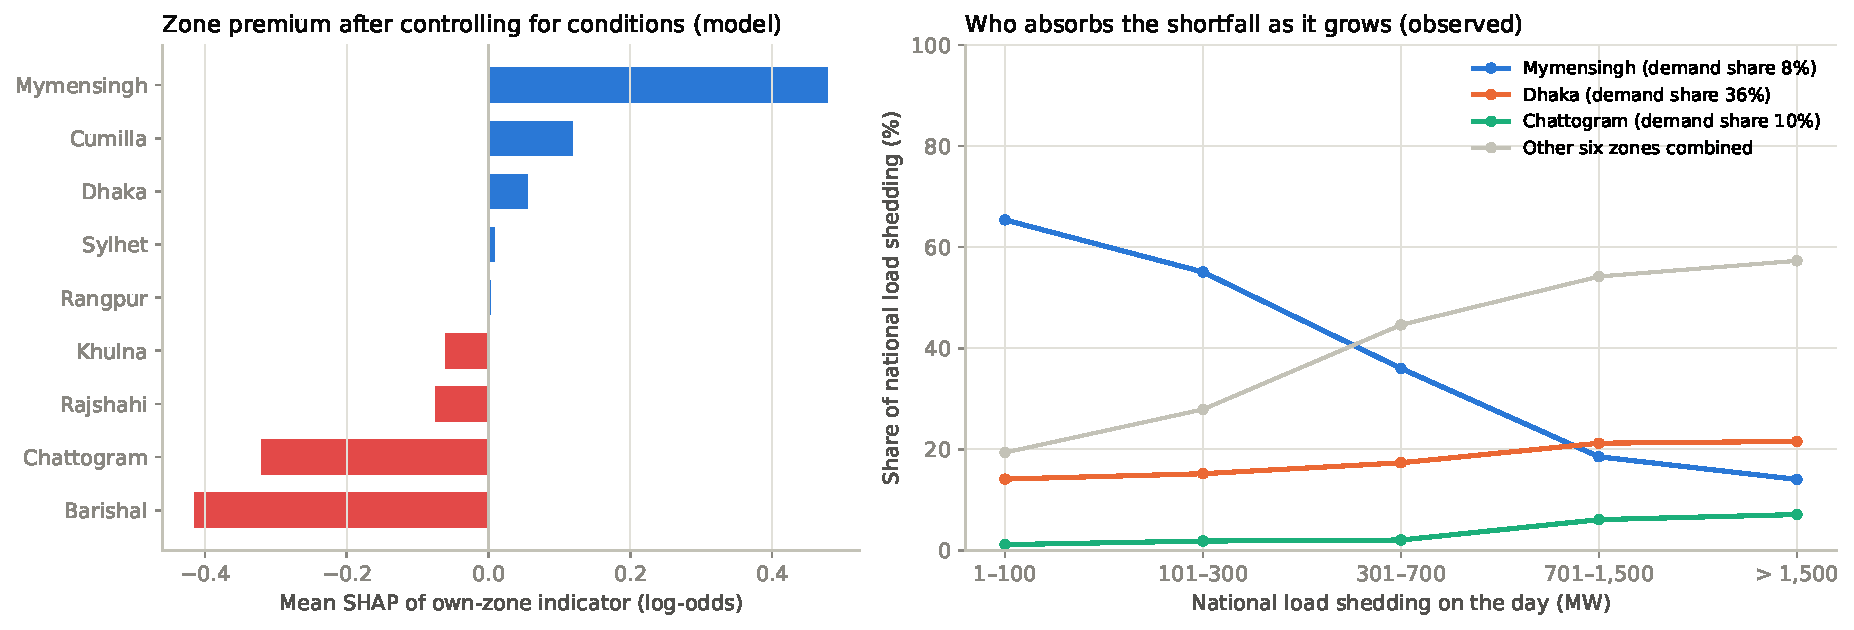
\includegraphics[width=\textwidth,height=0.72\textheight,keepaspectratio]{figures/fig43_zone_premium_and_share.pdf}}{Zone premium from the panel model (left) and observed share of national load shedding by national shortfall (right).}
\fi


\end{document}
